\documentclass[11pt,a4paper]{llncs}

%% margins
\usepackage{geometry}
\newgeometry{tmargin=2cm, bmargin=2cm, lmargin=2cm, rmargin=2cm}

%% various tools
\usepackage{amssymb}
\usepackage{graphicx}
\usepackage{amsmath}
%\usepackage{alltt}
%\usepackage{url}
\usepackage{listings}
\usepackage{booktabs}
\usepackage{color}

%% polish diacritic symbols and times new roman for the win
\usepackage{polski}
\usepackage[utf8]{inputenc}
\usepackage[T1]{fontenc}
%\usepackage{mathptmx}

%% algorithms
\usepackage{algpseudocode} 
\usepackage{algorithm}


\begin{document}


\mainmatter  

\title{Opracowanie koncepcji systemu do konstruowania dynamicznego słownika wielowyrazowych jednostek leksykalnych na podstawie korpusu tekstów}

\author{Michał Wendelberger, Bernadetta Maleszka}
\authorrunning{Michał Wendelberger, Bernadetta Maleszka}

\institute{Politechnika Wrocławska}

\maketitle

\begin{abstract}
W niniejszym raporcie zaprezentowano koncepcję systemu do konstruowania dynamicznego słownika wielowyrazowych jednostek leksykalnych na podstawie korpusu tekstów. Problem wydobywania jednostek wielowyrazowych jest rozważany w literaturze światowej, jednak nie istnieją narzędzia dedykowane dla języka polskiego. Proces budowy dynamicznego słownika został szczegółowo opisany w 6 krokach, w których zawiera się zarówno sama metoda ekstrakcji kolokacji, jak i zaproponowane podejście do badania wydobytych jednostek, dzięki którym możliwe jest doskonalenie opracowanych metod. Przeprowadzone badania eksperymentalne dają obiecujące wyniki.
\end{abstract}


\section{Wprowadzenie}

Celem niniejszego raportu jest przedstawienie prac realizowanych w ramach zadania A14 projektu \emph{,,Polska część infrastruktury naukowej CLARIN ERIC: Wspólne zasoby językowe i infrastruktura technologiczna''}. W zadaniu tym należy opracować system do wydobywania z tekstu opisanych strukturalnie, wielowyrazowych lematów języka polskiego z dużych zbiorów tekstów wyposażony we wzorcową ręcznie skonstruowaną bazę danych polskich wielowyrazowych lematów opisanych strukturalnie.

W raporcie została zaprezentowana koncepcja systemu do konstruowania dynamicznego słownika wielowyrazowych jednostek leksykalnych na podstawie korpusu tekstów. Jednostki wielowyrazowe to wyrażenia języka składające się z 2 lub więcej wyrazów, które wyróżniają się takimi własnościami jak niekompozycyjność składniowa i/lub semantyczna, często ustalona kolejność składników itp. Wydobywabie jednostek wielowyrazowych z tekstu jest istotne istotne dla praktycznych zastosowań przetwarzania języka naturalnego. Szczególnie ciekawym aspektem może być badanie, jak szybko jednostki wielowyrazowe zmieniają się w czasie i jak silnie zależą od dziedziny zastosowań.

Automatyczna ekstrakcja jednostek wielowyrazowych jest typowo przeprowadzana w oparciu o analizę statystyczną wystąpień słów w korpusie \cite{baldwin}. W pracy tej wzięto pod uwagę fakt, że wystąpienia słów mogą być nieciągłe, natomiast problemy swobodnego szyku wyrazów w zdaniu i bogatej fleksji są poruszane znacznie rzadziej, ze względu na to, że większość metod ekstrakcji została opracowana dla języka angielskiego. Bardziej zaawansowane metody używają automatycznej lematyzacji (sprowadzenia wyrazów do form podstawowych) i filtrowania potencjalnych kandydatów na kolokacje pod względem ich struktury składniowej.  

Autorzy pracy \cite{broda} zaproponowali podejście oparte na dwustopniowym procesie przetwarzania: po lematyzacji zostają zidentyfikowane proto-kolokacje (tj. wstępne kolokacje składające się z form podstawowych słów). Następnie dokonywana jest analiza statystyczna wystąpień proto-kolokacji w określonych wzorcach składniowych w korpusie tekstów. W wyniku otrzymywany jest opis binarnych jednostek wielowyrazowych wraz z ich opisami opartymi na ograniczeniach morfo-syntaktycznych.

W ramach wspomnianego zadania projektu CLARIN proponowane jest zbliżone podejście. Mianowicie, proces wydobywania kolokacji bazuje na statystycznych miarach częstości występowania ciągów słów, natomiast wydobyci w ten sposób kandydaci na jednostki wielowyrazowe są oceniane przez lingwistów. Do bazy jednostek zostają dodane te elementy, które zostały pozytywnie ocenione przez lingwistów. 

Niniejszy raport został podzielony w następujący sposób. Rozdział \ref{s2} zawiera informacje dotyczące narzędzi i oprogramowania, który wykorzystano do realizacji systemu. Szczegółowy opis procesu wydobywania jednostek został zawarty w rozdziale \ref{s3}. Zostały przedstawione również funkcjonalności dodatkowe, informacje dotyczące formatów wydobywanych jednostek wielowyrazowych oraz matematycznego modelu wykorzystanych funkcji. W rozdziale \ref{s4} zaprezentowano metodologię badań eksperymentalnych oraz wyniki pierwszych badań. Pracę podsumowano w rozdziale \ref{s5}.


\section{Narzędzie i oprogramowanie wykorzystane na potrzeby realizacji tematu}\label{s2}


\subsection{Biblioteka Corpus2}

Biblioteka \emph{Corpus2} to zestaw struktur danych i funkcji do przetwarzania korpusów, które są oznaczone morfo-syntaktycznie, z tagsetem pozycyjnym. 
Umożliwia ona wczytywanie i zapisywanie danych do różnych formatów danych takich jak \emph{XCES}, jego format rozszerzeny zwany \emph{CCL} czy formatów tekstowych takich jak przykładowo lekki format \emph{IOB-Chan}.
Opcjonalnie biblioteka wspiera także pracę, wczytywanie danych, z binarnym i zindeksowanym formatem \emph{Poliqarp} autorstwa pracowników instytutu \emph{Podstaw Informatyki Polskiej Akademii Nauk}, a opracowanym do przechowywania korpusów tekstowych.
Warto nadmienić, że biblioteka \emph{Corpus2} wspiera także wiele innych formatów plików.


 
Biblioteka została zaimplementowana w \emph{Instytucie Informatyki Politechniki Wrocławskiej} w języku \emph{C++}, ale powstały także skrypty w języku Python, opakowania, umożliwiające pracę z tą biblioteką z wykorzystaniem tego właśnie języka skryptowego.
Dodatkowo narzędzie jest dostępne nieodpłatnie na licencji \emph{GNU LGPL 3.0} lub w przypadku wykorzystania formatu \emph{Poliqarp} na licencji GNU GPL 3.0.



\emph{Corpus2} został wykorzystany w badaniach w ramach niniejszego projektu do wczytywania oznaczonych korpusów tekstowych z formatów \emph{IOB-Chan}, \emph{CCL} i \emph{Poliqarp}, a także do konwersji pomiędzy nimi.
Ponadto inne narzędzia wykorzystane w ramach zadania $A14$ także wykorzystują funkcjonalność tej biblioteki.


\subsection{Tagery WCRFT i WCRFT2}

Nazwa \emph{WCRFT} jest akronimem powstałym od słów \emph{Wrocław Conditional Random Fields Tagger} - wrocławskie narzędzie tagujące oparte o model matematyczny \emph{Conditional Random Field}.
\emph{WCRFT} został zaimplementowany z myślą o oznaczaniu tekstów języków fleksyjnych, zwłaszcza słowiańskich, a szczególnie języka polskiego.


Tager napisano w języku Python, z wykorzystaniem gotowej implementacji \emph{CRF} o nazwie \emph{CRF++}, która to napisana została w języku \emph{C++} \cite{wcrft}.
Narzędzie \emph{WCRFT} było implementowane głównie przez Adama Radziszewskiego.



\emph{WCRFT2} natomiast jest następcą tagera \emph{WCRFT}.
Został on napisany całkowicie w języku \emph{C++} -- zostało dokonane portowanie kodu z języka Python do języka \emph{C++}.
Taki zabieg pozwolił na usunięcie zależności związanych z językiem skryptowym, znaczne przyspiesznie tagera -- trzykrotne, a także usprawniło i ułatwiło proces budowy narzędzia.
Zaznaczyć trzeba, że po wykonaniu konwersji pomiędzy językami zachowano kompatybilność modeli z poprzednią wersją tagera, a wyniki dla obu wersji są takie same.
Ta wersja jest teraz zalecaną do użycia, a poprzednia nie jest już wspierana.



Narzędzie to, w celach badawczych na potrzeby projektu, zostało wykorzystane do oznaczenia morfo-syntaktycznego i ujednoznaczniania semantycznego słów z zebranych tekstów języka polskiego, które następnie zostały wykorzystane w procesie badania sposobów ekstrakcji kolokacji w tej pracy.
Do wykonania tych prac wykorzystany został nowy, gotowy model dla tagera udostępniony przez grupę G4.19.


\subsection{Formalizm WCCL}


\subsubsection{Wyjaśnienie terminu}
\emph{WCCL (Wrocław Corpus Constraint Language)} jest nowym formalizmem, językiem ograniczeń i narzędziem pozwalającym tworzyć wyrażenia funkcyjne, które można wykorzystać jako cechy, kluczowe informacje, dla wielu algorytmów przetwarzania języka naturalnego i maszynowego uczenia. 
Wyrażenia \emph{WCCL} działają na tekście uprzednio oznakowanego morfo-syntaktycznie na przykład za pomocą narzędzia wspomnianego we wcześniejszej części tej pracy -- tagera \emph{WCRFT2}. 
Chociaż formalizm ten był konstruowany z myślą o pracy z językiem polskim to według autorów powinien on także móc być użyty do pracy z innymi językami fleksyjnymi. 
Ograniczeniami mogą być jednak przyjęta tekstowa reprezentacja tagów oraz formaty oznakowanych korpusów, na których miałyby pracować wyrażenia \emph{WCCL} \cite[str. 1]{wccl}.



Omawiany język ograniczeń został zaimplementowany w języku \emph{C++} w postaci bibliotek wykorzystujących \emph{Corpus2} oraz system \emph{MACA (Morphological Analysis Converter and Aggregator)}. 
Dodatkowo napisane zostały także skrypty w języku Python opakowujące funkcjonalność \emph{WCCL} i umożliwiające prace z poziomu języka skryptowego, bez konieczności zaznajomienia się z językiem natywnym, w jakim formalizm ten został zaimplementowany. 
Dzięki temu tworzenie narzędzi i praca z \emph{WCCL} może być szybsza i prostsza. \cite[str. 3]{wccl}



Formalizm \emph{WCCL} został wykorzystany w badaniach z poziomu języka \emph{C++}, bez użycia opakowań, i posłuży głównie do filtrowania kandydatów na jednostki wielowyrazowe na podstawie części mowy składowych wyrażenia wielowyrazowego oraz innych cech takich jak przykładowo uzgodnienie rzeczownika z przymiotnikiem.
W ramach projektu zajmowano się badaniami nad kolokacjami w języku polskim, co rozwiązało ewentualne problemy mogące się pojawić przy pracy z innymi językami fleksyjnymi.


\subsubsection{Przykładowe wyrażenie}
Poniżej zaprezentowano przykładowy, prosty operator \emph{WCCL} zbliżony swoją składnią do operatorów stosowanych w niniejszych badaniach. 

\begin{lstlisting}[frame=single, tabsize=2, language=Python, caption=Przykładowe wyrażenie w języku \emph{WCCL}, captionpos=b, breaklines=true, basicstyle=\scriptsize]
@b:"SubstAdjOrSubstSubst"
(
	or
	(
		and
		(
			inter(class[0], {subst}),
			inter(class[1], {adj, subst}),
		
			setvar($Case, 0)
		),
		and
		(
			inter(class[1], {subst}),
			inter(class[0], {adj, subst}),
		
			setvar($Case, 1)
		)
	)
)
\end{lstlisting}

Powyższy listing prezentuje kod wyrażenia w języku \emph{WCCL}.
Składa się on z dwóch części - nagłówka i ciała.
Istotną informacją jest fakt, że operator \emph{WCCL} jest kontekstowy, wywoływany jest dla konkretnego miejsca w korpusie, jakiegoś wyrazu w nim zawartego.
Wyraz ten nazwijmy \emph{początkiem kontekstu operatora}.



Nagłówek zawiera dwie informacje o wyrażeniu, pierwsza z nich, \emph{@b}, to typ zwracany przez ten operator na podstawie wykonania instrukcji zawartych w jego ciele. 
Druga informacja to nazwa wyrażenia znajdująca się po dwukropku, tutaj będzie to \emph{SubstAdjOrSubstSubst}.
Powyższy kod zwróci jedną z dwóch wartości logicznych - \emph{True} lub \emph{False}.
Inne typy, które mogą zwracać operatory \emph{WCCL} to \emph{Position}, \emph{Set of strings} oraz \emph{Tagset symbol set}.
Pierwszy z nich to wartość całkowita - odpowiednik typu \emph{int} w języku \emph{C++}, drugi typ jest rozumiany jako zbiór ciągów znaków tekstowych, a trzeci to zestaw symboli używanego tagsetu.



Przed opisem ciała powyższego, przykładowego operatora należy wyjaśnić funkcje w nim użyte.
Pierwsze dwie z nich są intuicyjne - funkcja \emph{or} i \emph{and}.
Obie z nich zachowują się jak funkcje logiczne o tych samych nazwach anglojęzycznych, a argumenty dla nich są oddzielone przecinkiem tak samo jak w każdej funkcji języka \emph{WCCL}.
Funkcja \emph{setvar} ustawia wartość zmiennej o nazwie podanej w pierwszym argumencie na wartość zadaną parametrem drugim.
Natomiast funkcja \emph{inter} sprawdza przecięcie zbiorów zadanych jej argumentami i zwraca \emph{True} jeśli moc przecięcia jest niezerowa.
Kluczowa w tym wyrażeniu jest także funkcja \emph{class} przyjmująca tylko jeden argument typu całkowitego.
Funkcja ta zwróci klasę gramatyczną słowa oddalonego o zadaną argumentem liczbę wyrazów od \emph{początku kontekstu} tego wyrażenia.
Przykładowo przyjmijmy, że jakiś operator wywołuje kolejno funkcje \emph{class[-1]}, \emph{class[0]} i \emph{class[1]} na poniższym zdaniu, gdzie słowo będące \emph{początkiem kontekstu operatora} zostało oznaczone pogrubioną czcionką:
\begin{center}
Długie, ciężkie \textbf{spodnie} jeszcze się suszą.
\end{center}
Pierwsza funkcja z argumentem równym minus jeden zwróci klasę gramatyczną słowa \emph{ciężkie} czyli przymiotnik, druga klasę wyrazu będącego początkiem kontekstu operatora - \emph{spodnie}, czyli rzeczownik, natomiast wynikiem działania trzeciej dla wyrazu \emph{jeszcze} będzie partykuła.



Ciało powyższego wyrażenia \emph{WCCL} składa się z pojedynczego bloku - funkcji \emph{or}, sprawdzającej czy którykolwiek z dwóch bloków wewnętrznych \emph{and} zwróci wartość \emph{True} i jeśli tak to \emph{or} także zwróci \emph{True} jako wartość testu wykonanego przez ten operator.
Oba wewnętrzne bloki \emph{and} wykonują podobny test na dwóch kolejnych wyrazach z korpusu poczynając od \emph{początku kontekstu} wywołania wyrażenia.
Pierwszy blok \emph{and} sprawdza czy klasa gramatyczna słowa, dla którego operator został wywołany jest rzeczownikiem (\emph{subst}), a wyraz kolejny odpowiednio przymiotnikiem (\emph{adj}) lub też rzeczownikiem.
Jeśli obie funkcje \emph{inter} zwrócą \emph{True} to ustawiana jest zmienna, która potem może zostać odczytana w kodzie programu, który ten operator wywołał.
W przypadku omawianego operatora zmienna \emph{Case} będzie równa zero lub jeden w zależności od tego, która z funkcji \emph{and} zwróci wartość \emph{prawda} lub też może być niezdefiniowana jeśli obie funkcje \emph{and} zwrócą wartość \emph{fałsz}.
Zabieg taki pozwala przykładowo na określenie kolejności wyrazów, w jakiej wystąpiły w korpusie w celu odczytania tej informacji w programie.
Drugi blok \emph{and} zachowuje się analogicznie do pierwszego - sprawdza ten sam warunek, ale dla wyrazów ułożonych w odwrotnej kolejności.



Więcej informacji o wyrażeniach języka \emph{WCCL} można pozyskać zapoznając się z pracą \cite{wccl}.


\subsection{Słowosieć}

\emph{Słowosieć} jest polskim, podczas opisywania tego narzędzia drugim co wielkości na świecie \emph{Wordnetem} utworzonym i nieustannie rozwijanym przez \emph{Grupę Technologii Językowych Politechniki Wrocławskiej G4.19} w ramach projektów \emph{Clarin}, \emph{Synat} oraz \emph{Nekst} przy wsparciu uczelni oraz Ministerstwa Nauki i Szkolnictwa Wyższego.



Aktualna wersja \emph{Słowosieci} jest dostępna na darmowej licencji i zawiera 140 tysięcy słów, 200 tysięcy znaczeń oraz pół miliona relacji, jednak jest także szybko rozwijana przez jej pracowników i powyższe wartości mogą ulec znacznej zmianie w najbliższym wydaniu nowej wersji tego polskiego \emph{Wordnetu}.
Zawiera ona także 110 tysięcy haseł polsko-angielskich pozyskanych z \emph{Princeton Wordnet 3.1}.
Dostępnych jest także wiele publikacji traktujących o \emph{Słowosieci}, których spis dostępny jest na stronie internetowej \cite{slowosiec}.
Znaleźć tam można także dokładne statystyki, interfejs webowy oraz inne informacji tym o projekcie.



Baza danych polskiego \emph{Wordnetu} wykorzystywana była w celu pozyskania danych niezbędnych do oceny wyników badań przeprowadzonych w ramach niniejszego zadania.
% TODO a także w procesie filtorwania słów.


\subsection{SuperMatrix}

\emph{SuperMatrix} to pakiet wielu narzędzi zaimplementowanych w języku \emph{C++}, z założenia przystosowany do wykonywania różnych operacji na dwuelementowych obiektach takich jak przykładowo bi-gramy. 
Narzędzie to oferuje szereg funkcji, programów i gotowych algorytmów takich jak obliczanie wartości asocjacji z wykorzystaniem wielu miar - ponad osiemdziesięciu, wyliczanie wartości funkcji podobieństwa wierszy względem siebie, filtrowanie danych, transformacje, dzielenie macierzy, ich łącznie i inne.
Zawiera programy oraz skrypty umożliwiające budowanie krotek dwuelementowych i macierzy na kilka sposobów z korpusów tekstowych oznaczonych morfo-syntaktycznie.
Dla wygody i przyspieszenia pracy napisane zostały także opakowania w języku Python umożliwiające używanie bibliotek i narzędzi z pakietu \emph{SuperMatrix} z poziomu tego języka skryptowego.



Dużą zaletą omawianego narzędzia jest fakt, że było ono z powodzeniem wielokrotnie wykorzystywane, oraz że mimo dużej funkcjonalności jest ono dostępne na darmowej licencji.



Istotne jest, że dane składowane są w postaci macierzy dwuwymiarowej (podstawowego formatu danych dla narzędzi w tym pakiecie), co jest ograniczeniem i problemem w przypadku chęci pracy z kolokacjami dłuższymi niż dwuelementowe. 
Jednak zarówno to ograniczenie jak i fakt, że \emph{SuperMatrix} nie był projektowany do pracy z kolokacjami, nie jest problemem dla prowadzenia badań nad wyrażeniami dwuelementowymi. 
Wystarczy jedynie przygotować dane w odpowiedni sposób i wedle potrzeby, a następnie wykorzystać możliwości zawartych w pakiecie narzędzi.



Pierwsze badania na potrzeby tej pracy wykonywane były z wykorzystaniem właśnie tego pakietu narzędzi ze względu na liczność zaimplementowanych miar asocjacji, które można było zbadać bez konieczności przystosowywania narzędzia, implementacji nowych modułów pakietu, kolejnych programów czy całej aplikacji specjalnie do tego celu.
Badania te pozwoliły przetestować dziesiątki miar i ocenić, którymi z nich warto zająć się przy dalszej pracy z jednostkami wielowyrazowymi dłuższymi niż dwuelementowe.
Pierwsze wyniki nadały pewien kierunek dla prowadzania dalszych prac w temacie wyrażeń wielowyrazowych.


\subsection{MWeXtractor}

Pakiet narzędzi \emph{SuperMatrix} z założenia miał być wykorzystywany do pracy z parami elementów, z których jeden jest reprezentowany danymi zawartymi w wierszu, a drugi w kolumnie macierzy.
Cecha ta jest swoistego rodzaju ograniczeniem i problemem uniemożliwiającym, a przynajmniej bardzo utrudniającym prowadzenie badań obiektów składających się z trzech lub większej liczby elementów.
Sposób przechowywania danych i ich wykorzystania musiałby zostać przygotowany do składowania w formacie pakietu \emph{SuperMatrix} czyli dwuwymiarowej macierzy, co znacząco utrudniałoby wykonanie zadania.
Dodatkowo zabieg ten wydaje się zły koncepcyjnie -- to format danych powinien być dopasowany do składowania określonych danych, a nie dane upakowane na siłę w taki sposób, aby zmieściły się w narzuconym formacie niebędącym przygotowanym do przechowywania informacji tego rodzaju.
Sam sposób przechowywania danych był jednak tylko wierzchołkiem góry lodowej.
Praktycznie wszystkie narzędzia pakietu \emph{SuperMatrix} zostały przygotowane do pracy z obiektami dwuelementowymi.
Fakt ten oznacza, że wykorzystanie omawianego narzędzia byłoby niewielką wartością dodaną w prowadzeniu badań, ponieważ dużą część funkcjonalności trzeba byłoby zaimplementować od nowa mając na uwadze ograniczenia i koncepcje wprowadzone na potrzeby realizacji projektu \emph{Supermatrix}.
Reimplementacja metod wymagana byłaby także ze względu na wspomnianą wcześniej konieczność upakowania danych $N$-elementowych do postaci dwuelementowej.
Mogłoby to doprowadzić do poświęcenia dużej ilości czasu i uwagi na zaplanowanie, dostosowanie, implementację i integrację nowych fragmentów oprogramowania \emph{SuperMatrix} zamiast wykorzystania tych zasobów do realizacji faktycznego zadania projektu.



Omówione problemy były jednymi z głównych przyczyn opracowania nowego narzędzia, niezależnego od pakietu \emph{SuperMatrix}, specjalizowanego pod kątem prowadzania badań dotyczących wyrażeń wielowyrazowych, między innymi na potrzeby niniejszej pracy.
Narzędzie \emph{MWeXtractor} utworzone przez autora tej pracy jest biblioteką progrmaistyczną oraz pakietem struktur danych, programów, skryptów i niewielkiej ilości danych.
Posłużyło ono do prowadzenia badań nad kolokacjami, których wyniki zostały zamieszczone w dalszej części niniejszej pracy.



Większość oprogramowania, a w szczególności jego główne funkcjonalności zostały zaimplementowane w języku \emph{C++} w celu osiągnięcia jak największej wydajności pamięciowej odnośnie składowania danych oraz obliczeniowej narzędzi i algorytmów.
Wykorzystany standard tego języka to \emph{C++11}.
Język skryptowy \emph{Python} został wykorzystany do utworzenia części oprogramowania pomocniczego -- skryptów.
Oprogramowanie związane z algorytmem genetycznym pochodzi z kodów zaimplementowanych przez Łukasza Kłyka \cite{klyk}, które zostało dostosowane do współpracy z pakietem narzędzi \emph{MWeXtractor}.


\section{Przykładowe schematy użytkowania narzędzia}\label{s3}
Dwie typowe ścieżki przetwarzania umożliwione przez oprogramowanie \emph{MWeXtractor} zostały opisane w dalszej części niniejszej pracy.
Pierwsza z nich jest związana z badaniem jakości funkcji asocjacyjnych i klasyfikatorów, a druga służy do ekstrakcji kolokacji z korpusów tekstowych.

\subsection{Schemat procesu badania metod ekstrakcji kolokacji}
Schemat \ref{user_processing_scheme_research} prezentuje pierwszą z dwóch typowych ścieżek przetwarzania, odpowiedzialną za badania metod ekstrakcji wyrażeń wielowyrazowych.

\begin{figure}[h!]
\centering
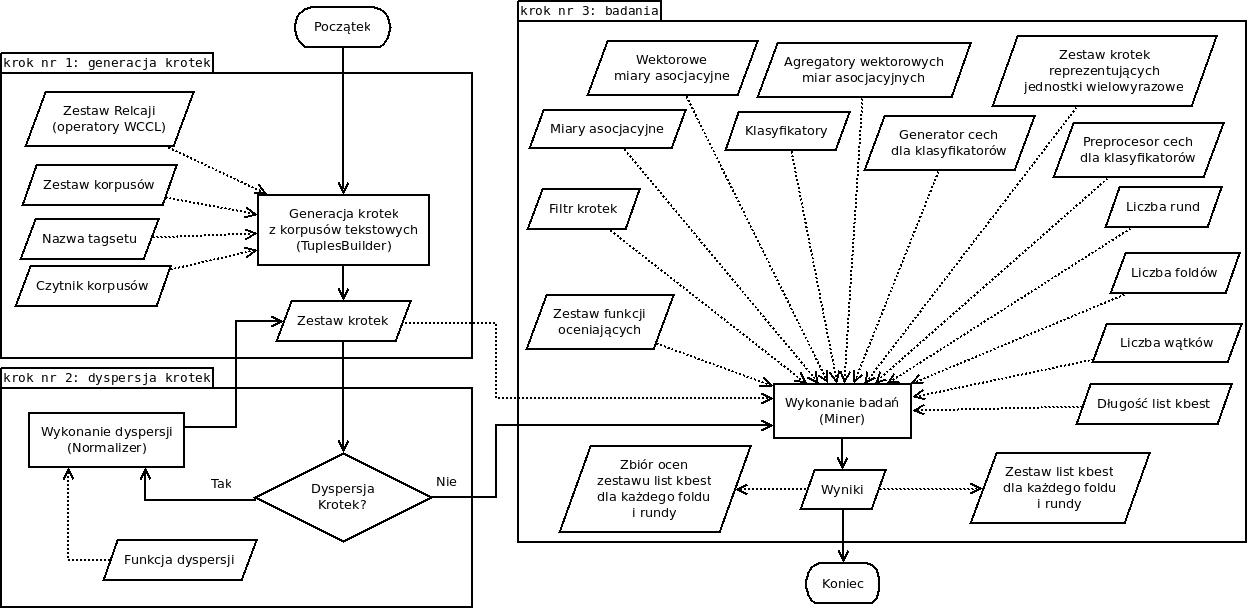
\includegraphics[width=\textwidth]{charts/user_processing_scheme_research.jpg}
\caption [Przykładowy schemat procesu badania jakości rankerów]{Powyższy schemat prezentuje jeden z typowych procesów użytkowania oprogramowania \emph{MWeXtractor} -- badania jakości generowanych przez rankery kolokacji}
\label{user_processing_scheme_research}
\end{figure}


\noindent\textbf{Krok numer 1: generacja krotek}


Najpierw należy przygotować listę korpusów, z których mają zostać wydobyte dane do przeprowadzenia badań nad metodami ekstrakcji wyrażeń wielowyrazowych.
Należy podać typ czytnika korpusów oraz tagset jakim dane tekstowe zostały opisane.
Następnie zdefiniować zestaw relacji -- operatorów zapisanych w języku \emph{WCCL}, które specyfikują jakich kandydatów na wyrażenia wielowyrazowe należy wyszukiwać w badanych korpusach tekstowych.
Dzięki nim można ograniczyć zestaw kandydatów, nad którymi chce się prowadzić badania.
Jeśli użytkownik jest zainteresowany wszystkimi możliwymi do utworzenia n-gramami może przykładowo wykorzystać do tego celu operator \emph{WCCL} generujący wszystkie możliwe kombinacje n-elementowe.
Zaznaczyć trzeba, że wydobywani kandydaci na kolokacje nie muszą być ciągli, a ich szyk może być zmienny, wszystko zależy od tego jak zostaną przygotowane relacje.
Tak przygotowany zestaw danych i parametrów należy następnie podać jako argumenty dla programu \emph{TuplesBuilder}, który na ich podstawie przygotuje skład krotek -- podstawową strukturę danych dla oprogramowania \emph{MWeXtractor} składującą krotki.


\noindent\textbf{Krok numer 2: dyspersja krotek}


Drugi krok tego schematu przetwarzania jest opcjonalny i dotyczy modyfikacji informacji o zebranych krotkach -- ich częstości będących kluczowym elementem związanym z późniejszą oceną kandydatów na kolokacje.
Do tego celu wykorzystana może zostać jedna z funkcji dyspersji zaimplementowana w tym celu, zostaną one opisane w dalszej części tej pracy.
Zależnie od wybranej metody dyspersji pod uwagę są brane różne statystyki związane z krotkami, przykładowo będą to częstości danych krotek, liczba krotek w danym korpusie czy informacja o tym w ile korpusach dana krotka została odnaleziona.
W skrócie, miara dyspersji ma za zadanie zmienić rozkład częstości krotek w składzie promując instancje ciekawe -- mniej typowe.
\par
Jednak z zaimplementowanych funkcji dyspersji -- \emph{Lynes D3}, bazuje na mierze $ Hi^{2} $, a tym samym potrzebne są jej pewne dane statystyczne.
Jeśli ta miara ma zostać wykorzystana do dyspersji krotek to trzeba jej te dane statystyczne przygotować.
Sposób generacji tych informacji został opisany w trzecim kroku omawiania kolejnego z przykładowych schematów przetwarzania.
Zaznaczyć jednak trzeba, że ta miara to wyjątek.


\noindent\textbf{Krok numer 3: badania}


Niniejszy krok jest krokiem finalnym tej ścieżki przetwarzania.
Polega on na wykonaniu r-rundowej, f-foldowej walidacji krzyżowej dla danego zbioru danych, z wykorzystaniem określonych miar asocjacyjnych i klasyfikatorów.
Oprogramowanie przeznaczone do tego celu zostało nazwane \emph{Miner}.
Wyniki wygenerowane przez ten program zostają poddane ocenie przez użytkownika narzędzi \emph{MWeXtractor}. 
Do łączenia dużych zestawów wyników przygotowany został skrypt w języku \emph{Python} uśredniający wyniki dla wszystkich z foldów z każdej z rund, dla poszczególnych funkcji rankingowych z osobna.
Pozwala to na szybkie wygenerowanie zbiorczych wyników i przykładowo utworzenie wykresów prezentujących jakości rezultatów zastosowanych metod wydobycia według określonych miar.
\par
Parametry programu \emph{Miner} zostały wymienione i opisane w poniższej tabeli \ref{miner_parameters}:

\begin{table}[h!]
\centering
\begin{tabular}{l | l | p{0.6\linewidth}}
	\toprule 
	Nazwa & Typ & Opis \\
	\midrule 
	Skład krotek & nazwa folderu & ścieżka do folderu ze składem krotek \\ 
	\hline
	Wyjście programu & nazwa folderu & ścieżka do folderu, w którym zostaną zamieszczone wyniki\\ 
	\hline
	Miary asocjacji & ciągi tekstowe & parametr wielokrotny, tekst reprezentujący funkcje asocjacyjną, którą program ma wykorzystać\\ 
	\hline
	Miary wektorowe & ciągi tekstowe & parametr wielokrotny, tekst reprezentujący wektorową miarę asocjacyjną, którą program ma wykorzystać\\ 
	\hline
	Agregatory & ciągi tekstowe & parametr wielokrotny, tekst reprezentujący funkcję agregującą wyniki miar wektorowych, po jednej funkcji dla każdej z nich\\
	\hline
	Klasyfikatory & ciągi tekstowe & parametr wielokrotny, tekst reprezentujący klasyfikator, który program ma wykorzystać\\ 
	\hline
	Generator cech & ciąg tekstowy & wektorowa miara asocjacyjna, która zostanie wykorzystana jako generator cech dla klasyfikatorów\\ 
	\hline
	Preprocesor cech & ciąg tekstowy & parametr opcjonalny, tekst reprezentujący funkcję, która ma zostać wykorzystana do normalizacji cech\\ 
	\hline
	Zestaw JW & nazwa pliku & plik zawierający w każdej linii ciąg wyrazów oddzielonych spacjami, reprezentujący wyrażenie wielowyrazowe\\ 
	\hline
	Funkcje oceny & ciągi tekstowe & parametr wielokrotny, tekst reprezentujący funkcję oceny, którą program ma wykorzystać\\ 
	\hline
	Filtr krotek & ciąg tekstowy & tekst reprezentujący filtr, który program ma wykorzystać do wyznaczenia zestawu krotek, z których ma korzystać i, dla których wygenerować dane\\ 
	\hline
	Liczba wątków & liczba całkowita & maksymalna liczba wątków do wykorzystania przez program\\ 
	\hline
	Liczba rund & liczba całkowita & liczba rund walidacji krzyżowej\\ 
	\hline
	Liczba foldów & liczba całkowita & liczba foldów dla każdej walidacji krzyżowej\\
	\bottomrule
\end{tabular}
\caption[Parametry programu \emph{Miner}]{Tabela zawiera nazwy, typy oraz opisy parametrów wykorzystywanych przez program \emph{Miner}}
\label{miner_parameters}
\end{table}

\par
Wspomniany zbiór wyników jest obszerny, podzielony na pliki, których są dwa rodzaje - pliki z listami k-najlepszych kandydatów na wyrażenia wielowyrazowe, oraz pliki z ocenami tych list.
Liczba wygenerowanych plików rankingowych jest równa \( ((A + V + C) * R * F) \), gdzie \emph{A}, \emph{V} oraz \emph{C} oznaczają kolejno liczbę wykorzystanych funkcji asocjacyjnych, wektorowych miar asocjacyjnych oraz klasyfikatorów, natomiast \emph{R} i \emph{F} to kolejno liczba rund i foldów walidacji krzyżowej.
Dodatkowo dla każdego pliku z rankingiem wygenerowanych zostaje \emph{Q} plików oceny tego rankingu, gdzie \emph{Q} jest liczbą wykorzystanych funkcji oceny list k-najlepszych.
Wzorzec nazwy pliku z rankingiem jest generowany w sposób następujący: \emph{kbest.nr\_rankera.nr\_rundy.nr\_foldu.csv}, natomiast wzorzec dla plików z wynikami funkcji oceny list k-najlepszych to: \emph{kbest.nr\_rankera.nr\_rundy.nr\_foldu.nr\_funkcji\_oceny.csv}.
Numer rankera jest z przedziału:
\begin{enumerate}
  \item \texttt{[0     : A         - 1]} - dla funkcji asocjacyjnych;
  \item \texttt{[A     : A + V     - 1]} - dla wektorowych miar asocjacyjnych;
  \item \texttt{[A + V : A + V + C - 1]} - dla klasyfikatorów.
\end{enumerate}

Ze względu na dużą liczbę plików wynikowych zaimplementowany został skrypt wspomniany wcześniej, łączący wyniki poprzez uśrednienie wyników dla każdego foldu z każdej rundy dla poszczególnych funkcji rankingujących z osobna i generuje pojedynczy plik z jedną kolumną dla każdego rankera.
Skrypt nazwany został \emph{cv\_quality\_merger.py}, został napisany w języku \emph{Python} i jest częścią pakietu \emph{MWeXtractor}.


\subsection{Schemat procesu ekstrakcji wyrażeń wielowyrazowych}
Schemat \ref{user_processing_scheme_extraction} prezentuje pierwszą z dwóch typowych ścieżek przetwarzania, odpowiedzialną za badanianie metod ekstrakcji wyrażeń wielowyrazowych.

\begin{figure}[h!]
\centering
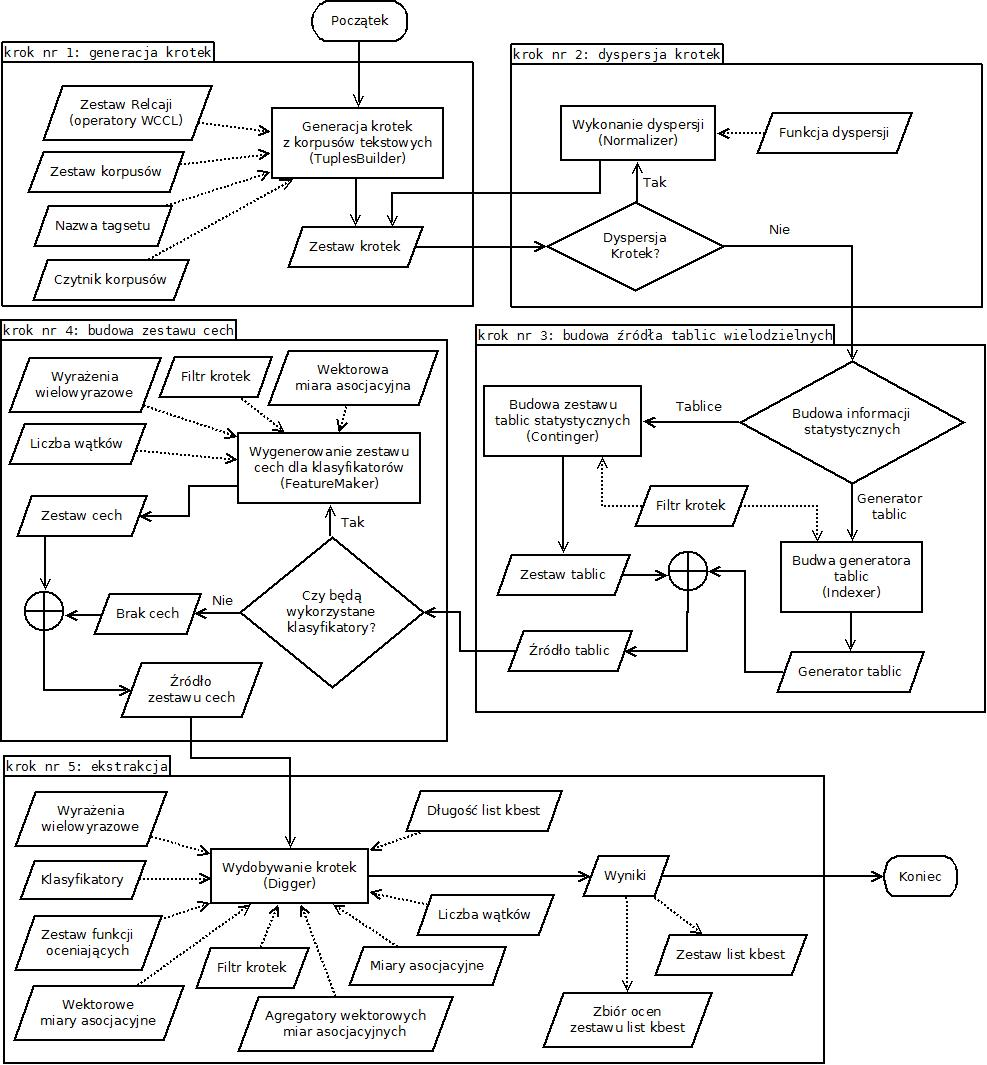
\includegraphics[width=\textwidth]{charts/user_processing_scheme_extraction.jpg}
\caption [Przykładowy schemat procesu wydobywania wyrażeń wielowyrazowych]{Powyższy schemat prezentuje jeden z typowych procesów wydobywania wyrażeń wielowyrazowych za pomocą oprogramowania \emph{MWeXtractor}}
\label{user_processing_scheme_extraction}
\end{figure}


\noindent\textbf{Kroki numer 1 i 2}


Oba krotki są takie same jak w przypadku poprzedniego przykładowego schematu przetwarzania -- badania miar asocjacyjnych i klasyfikatorów.


\noindent\textbf{Krok numer 3: budowa źródła tablic wielodzielnych}


Prawie wszystkie zaimplementowane miary i klasyfikatory korzystają z informacji zawartych w tablicach wielodzielnych dla krotek. 
Miary korzystają z tych informacji bezpośrednio do obliczania wartości dla kolokacji, a w przypadku klasyfikatorów miary te wykorzystywane są do generowania cech instancji.
Wyjątkiem są miary oparte na szyku, ponieważ nie korzystają takich informacji.
Krok trzeci polega na utworzeniu jednego z dwóch dostępnych źródeł tablic -- ich generatora lub składu. 
Programy przygotowane do wykonania tego zadania to odpowiednio \emph{Indexer} oraz \emph{Continger}.
Zazwyczaj generator tablic zajmuje znacznie mniej pamięci operacyjnej -- kilkakrotnie mniej, ale odwołanie do tablic wielodzielnych jest znacznie wolniejsze niż w przypadku składu tablic, ponieważ generator tworzy je na bieżąco, a skład przechowuje już gotowe tablice.
Zestaw krotek, na podstawie których źródło tablic ma zostać wygenerowane można ograniczyć za pomocą filtrów.
Zabieg taki pozwala na używanie określonego składu krotek do różnych celów, bez konieczności wydobywania kandydatów z korpusów wielokrotnie.
Dodatkowo umożliwia to zbudowanie informacji statystycznych na podstawie innego zestawu krotek niż ten, z którego wyrażenia wielowyrazowe mają być wydobywane.
Jako praktyczny przykład takiego zadania można podać ten, w którym informacja statystyczna budowana jest na podstawie krotek zebranych za pomocą relacji okna, a wydobywanie wyrażeń wielowyrazowych jedynie na podstawie innych relacji, przykładowo o określonych wzorcach strukturalnych.


\noindent\textbf{Krok numer 4: budowanie zestawu cech}


Niniejszy krok jest opcjonalny i może zostać pominięty jeśli użytkownik nie ma zamiaru korzystać z klasyfikatorów.
Jeśli jednak użytkownik będzie chciał skorzystać z klasyfikatorów lub wygenerować zestaw cech, z który będzie można wykorzystać w oprogramowaniu \emph{WEKA} to może do tego celu użyć programu o nazwie \emph{FeatureMaker}.
Zadaniem tego modułu jest wygenerowanie cech dla kandydatów na kolokacje, spośród których mają być w przyszłości wydobyte wyrażenia wielowyrazowe.
Do wykonania tego zadania generator cech wykorzystuje miary asocjacyjne, których wyniki traktowane są jako cechy.
Dopuszczalne jest także wykorzystanie uprzednio wyuczonych klasyfikatorów, przykładowo sieci neuronowych, do generowania cech opisujących kandydatów.
Zestaw kandydatów można ograniczyć za pomocą filtru jeśli nie ma potrzeby wyznaczenia cech dla wszystkich krotek.
\par
Aktualnie jedynym wspieranym formatem pliku wykorzystywanym do zapisu zestawu cech w pamięci nieulotnej jest \emph{ARFF}.
\par
Zamieszczona poniżej tabela \ref{feature_maker_parameters} zawiera opisy parametrów programu \emph{FeatureMaker}:
\begin{table}[h!]
\centering
\begin{tabular}{l | l | p{0.6\linewidth}}
	\toprule 
	Nazwa & Typ & Opis \\
	\midrule 
	Skład krotek & nazwa folderu & ścieżka do folderu ze składem krotek \\ 
	\hline
	Wyjście programu & nazwa pliku & ścieżka do pliku, w którym zostaną zapisane wyniki\\ 
	\hline
	Zestaw JW & nazwa pliku & plik zawierający w każdej linii ciąg wyrazów oddzielonych spacjami, reprezentujący wyrażenie wielowyrazowe, wykorzystany w przypisywaniu klas krotkom\\ 
	\hline
	Generator cech & ciągi tekstowe & tekst reprezentujący wektorową miarę asocjacyjną, którą program ma wykorzystać do generowania cech dla krotek\\ 
	\hline
	Filtr krotek & ciąg tekstowy & tekst reprezentujący filtr, który program ma wykorzystać do wyznaczenia zestawu krotek, dla których wygenerować cechy\\ 
	\hline
	Liczba wątków & liczba całkowita & maksymalna liczba wątków do wykorzystania przez program\\ 
	\bottomrule
\end{tabular}
\caption[Parametry programu \emph{FeatureMaker}]{Tabela zawiera nazwy, typy oraz opisy parametrów wykorzystywanych przez program \emph{FeatureMaker}}
\label{feature_maker_parameters}
\end{table}


\noindent\textbf{Krok numer 5: ekstrakcja}


% TODO: Digger modifications: classifiers + features + output
Ostatnim krokiem tej ścieżki przetwarzania jest wykorzystanie wcześniej utworzonych danych do ekstrakcji wyrażeń wielowyrazowych z korpusów tekstowych.
Zadanie to może zostać wykonane za pomocą programu \emph{Digger}.
Zestaw parametrów programu jest zbliżony do tych dla narzędzie \emph{Miner}, w poniższej tabeli \ref{digger_parameters} opisane zostały argumenty dla oprogramowania \emph{Digger}:

\begin{table}[h!]
\centering
\begin{tabular}{l | l | p{0.6\linewidth}}
	\toprule 
	Nazwa & Typ & Opis \\
	\midrule 
	Skład krotek & nazwa folderu & ścieżka do folderu ze składem krotek \\ 
	\hline
	Źródło tablic & nazwa pliku & ścieżka do pliku ze składem lub generatorem krotek\\
	\hline
	Wyjście programu & nazwa folderu & ścieżka do folderu, w którym zostaną zamieszczone wyniki\\ 
	\hline
	Miary asocjacji & ciągi tekstowe & parametr wielokrotny, tekst reprezentujący funkcje asocjacyjną, którą program ma wykorzystać\\ 
	\hline
	Miary wektorowe & ciągi tekstowe & parametr wielokrotny, tekst reprezentujący wektorową miarę asocjacyjną, którą program ma wykorzystać\\ 
	\hline
	Agregatory & ciągi tekstowe & parametr wielokrotny, tekst reprezentujący funkcję agregującą wyniki miar wektorowych, po jednej funkcji dla każdej z nich\\
	\hline
	Klasyfikatory & ciągi tekstowe & parametr wielokrotny, tekst reprezentujący klasyfikator, który program ma wykorzystać\\ 
	\hline
	Źródło cech & nazwa pliku & Źródło zestawu cech dla krotek\\ 
	\hline 
	Zestaw JW & nazwa pliku & plik zawierający w każdej linii ciąg wyrazów oddzielonych spacjami, reprezentujący wyrażenie wielowyrazowe\\ 
	\hline
	Funkcje oceny & ciągi tekstowe & parametr wielokrotny, tekst reprezentujący funkcję oceny, którą program ma wykorzystać\\ 
	\hline
	Filtr krotek & ciąg tekstowy & tekst reprezentujący filtr, który program ma wykorzystać do wyznaczenia zestawu krotek, z których ma korzystać i, dla których wygenerować dane\\ 
	\hline
	Liczba wątków & liczba całkowita & maksymalna liczba wątków do wykorzystania przez program\\ 
	\bottomrule
\end{tabular}
\caption[Parametry programu \emph{Digger}]{Tabela zawiera nazwy, typy oraz opisy parametrów wykorzystywanych przez program \emph{Digger}}
\label{digger_parameters}
\end{table}

Zestaw generowanych wyników jest podobny do tego generowanego przez narzędzie \emph{Miner}, ale jest mniejszy, ponieważ nie ma podziału na rundy i foldy ze względu na brak walidacji krzyżowej.
Wzorce nazw dla plików k-najlepszych krotek i plików z ocenami dla tych list prezentują się teraz następująco: \emph{kbest.nr\_rankera.csv} oraz \emph{quality.nr\_rankera.nr\_funkcji\_oceny.csv}.
Zasada generowania numeru rankera jest taka sama jak w przypadku programu \emph{Miner}.


\subsection{Schemat koncepcyjny narzędzia sieciowego do ekstrakcji kolokacji}
Poniższy schemat \ref{web_tool} przedstawia koncepcję działania narzędzia sieciowego.

\begin{figure}[h!]
\centering
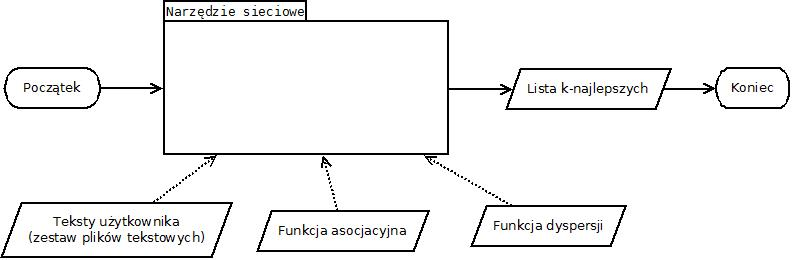
\includegraphics[width=\textwidth]{charts/web_tool.jpg}
\caption [Schemat działania narzędzia sieciowego]{Schemat działania narzędzia sieciowego}
\label{web_tool}
\end{figure}


\subsection{Funkcjonalności dodatkowe}
Pakiet narzędzi \emph{MWeXtractor} posiada też dodatkowe funkcjonalności, z których część została opisana w tej części niniejszej pracy.


\noindent\textbf{Program \textit{Cover}}


Program nazwany \emph{Cover} służy do weryfikacji relacji oraz badania przecięcia zbioru wydobytych krotek pomiędzy relacjami -- sprawdzenie jak dużo z nich zostało przyporządkowanych do więcej niż jednej relacji.
Praktyczne wykorzystanie tego oprogramowania to sprawdzenie pokrycia wzajemnego operatorów \emph{WCCL} zastosowanych do wydobywania krotek z tekstów.
Wynikiem jego działania jest macierz kwadratowa o wymiarze równym liczbie relacji wykorzystanych w procesie tworzenia \emph{składu krotek}, gdzie każdy z wierszy i każda z kolumn mają przypisaną do siebie określoną nazwę operatora \emph{WCCL}.
Liczby całkowite zapisane na przecięciu wierszy z kolumnami informują ile różnych krotek zostało przypisanych zarówno do relacji będącej etykietą wiersza jak i kolumny.
Interpretacją liczby na przecięciu wiersza i kolumny -- diagonali, odpowiadającym tej samej relacji jest informacja ile krotek zostało zakwalifikowanych do tej relacji.
Jeśli w danym wierszu lub kolumnie wystąpi więcej niż jedna wartość większa od zera poza polem na diagonali macierzy oznacza to, że relacje są nierozłączne -- część krotek przyporządkowano do więcej niż jednej relacji.
Należy jednak pamiętać, że narzędzie to nie jest wyrocznią, ponieważ jeśli dla danego zbioru danych okaże się, że relacje są rozłączne to nie oznacza to, że dla innego zbioru, większego czy lepiej oddającego rzeczywistość, sytuacja się powtórzy.
Zbudowana w ten sposób macierz jest symetryczna.
\par
Opisywany tutaj program \emph{Cover} ma także drugie zastosowanie wspomniane we wcześniejszej części tego fragmentu niniejszej pracy -- badanie przecięcia zbioru krotek ze składu i tego zadanego parametrem programu.
Na podstawie zadanego pliku z ciągami wyrazów program bada ile z nich, oraz które konkretnie ciągi zostały odnalezione w \emph{składzie krotek}.
Funkcjonalność ta może posłużyć przykładowo do wyznaczania zbioru krotek pozytywnych, czyli wyrażeń wielowyrazowych, które zostały w tym tekście odnalezione podczas wydobywania kandydatów na kolokacje.
Dodatkowo zakres poszukiwań wśród krotek w składzie można zawęzić za pomocą filtru.
Zabieg taki pozwala na lepsze poznanie zbioru danych.


\noindent\textbf{Wydobywanie form napotkanych}


Program \emph{Digger} umożliwia dodatkowo wydobycie form napotkanych dla krotek z wygenerowanych list k-najlepszych kandydatów na kolokacje.
Jeśli użytkownik jest zainteresowany ekstrakcją form napotkanych to powinien podać cztery dodatkowe parametry dla tego programu, które zostały opisane w poniższej tabeli \ref{digger_parameters_orths}:

\begin{table}[h!]
\centering
\begin{tabular}{l | l | p{0.5\linewidth}}
	\toprule 
	Nazwa & Typ & Opis \\
	\midrule 
	Zestaw korpusów & nazwa pliku & ścieżka do pliku zawierającego listę ścieżek do korpusów, po jednej ścieżce w każdej linii pliku \\ 
	\hline
	Operatory WCCL & nazwa pliku & ścieżka do pliku z operatorami języka \emph{WCCL}, które były użyte przy wydobywaniu kandydatów na kolokacje w kroku numer jeden\\ 
	\hline
	Tagset & ciąg znaków & nazwa wykorzystanego tagsetu w korpusach \\
	\hline
	Czytnik & ciąg znaków & nazwa czytnika korpusów\\
	\bottomrule
\end{tabular}
\caption[Parametery dodatkowe programu \emph{Digger}]{Tabela zawiera nazwy, typy oraz opisy parametrów dodatkowych wykorzystywanych przez program \emph{Digger}}
\label{digger_parameters_orths}
\end{table}

Wyekstrahowany zestaw form napotkanych dla krotek zostanie zapisany w pojedynczym pliku w formacie \emph{csv}.
Format pliku jest następujący: najpierw zapisana zostaje reprezentacja krotki z jednej z list k-najlepszych, a część kolejnych linii rozpoczyna się tabulacją i zawiera ciąg wyrazów napotkanych dla tej krotki, wraz z jego częstością.
Następnie zapis taki się powtarza dla wszystkich wydobytych krotek jeśli jest ich więcej, ale bez powtórzeń jeśli krotki wystąpiły na różnych listach k-najlepszych.
Dodatkowo napisany został skrypt łączący listy k-najlepszych z zestawem wydobytych dla nich form napotkanych i tworzy nowe listy k-najlepszych zachowując kolejność rankingu i przypisując do każdej pozycji zestaw forma napotkanych tej krotki wraz częstościami tych forma napotkanych.
Kolejność form napotkanych po łączeniu będzie posortowana malejąco po ich częstościach.
Skrypt ten napisany w języku \emph{Python} został nazwany \emph{kbest\_orth\_merger.py} i jest częścią pakietu \emph{MWeXtractor}.


\subsection{Format składowania danych zebranych z korpusów}
Jako format przechowywania danych wykorzystano krotki o różnych długościach\footnote{Długość krotki rozumiana jest jako liczba jej elementów składowych, przykładowo wyrazów.}, co umożliwia składowanie informacji o wyrażeniach wielowyrazowych dowolnej długości w intuicyjny sposób.
Krotki są dość powszechnym, elastycznym i prostym formatem stosowanym do przechowywania danych, a dodatkowo zapisywane są w postaci tekstu czytelnego dla człowieka, co czyni format przejrzystym, łatwym do ewentualnej edycji i ułatwia analizę zapisanych informacji.


Krotka reprezentująca wyrażenie wielowyrazowe zawiera w sobie słowa w ustalonej kolejności wraz z ich częściami mowy, które wchodzą w skład tego wyrażenia.
Każda z krotek zawiera także informację w jakiej relacji wystąpiły zawarte w tej krotce wyrazy.
Relacja jest jednym z operatorów \emph{WCCL} wykorzystanym w procesie tworzenia krotek na podstawie korpusów - proces ten został opisany w dalszej części tej sekcji.
Jeśli dane zestawienie wyrazów w tekście spełnia wymagania dla kilku różnych wyrażeń języka ograniczeń to dla każdego z nich powstanie osobna krotka zawierająca te same elementy, ale różniąca się relacją.
Dodatkowo w krotce zawarte są także metadane o niej, takie jak jej częstość\footnote{Częstość krotki określa liczbę wystąpień konkretnego zestawienia słów w danej relacji.} w przetworzonych korpusach danych.
Relacja nie jest uwzględniana w rozmiarze krotki.
Format składowania krotek w pliku tekstowym wraz z przykładem został zamieszczony w tabeli \ref{tuple_format}.

\begin{table}[h!]
\centering
\begin{tabular}{c|c|c|c|c|c}
\toprule
	\textbf{nazwa relacji} & 
		\textbf{arność relacji} & 
		\textbf{częstość krotki} & 
		\textbf{cz.m.:s1} & 
		\textbf{cz.m.:s2} & 
		\ldots \\
	\midrule
	AdjSubst & 2 & 17 & adj:nowy & subst:but & \\
\bottomrule
\end{tabular}
\caption[Format składowania krotek w pliku tekstowym]{Format składowania krotek w pliku tekstowym wraz z przykładem. Elementy (ciągi znakowe) składowane w pliku tekstowym oddzielone są od siebie tabulatorami. Arność relacji jest tożsama z rozmiarem krotki. Skrótowiec \emph{cz.m:sN} pochodzi od: część mowy, dwukropek, \emph{N}-te słowo krotki.}
\label{tuple_format}
\end{table}


Istotnym elementem przetwarzania tak dużych zbiorów danych jest wydajny sposób składowania ich w pamięci operacyjnej maszyny przetwarzającej.
Do tego celu opracowana, zaimplementowana i wykorzystana została struktura starająca się minimalizować zużycie pamięci przy zachowaniu szybkiego dostępu do danych poprzez wykorzystanie implementacji zbiorów opartych o drzewa czerwono-czarne i funkcje skrótu\footnote{Popularna nazwa anglojęzyczna to \emph{hash function} -- funkcja haszująca.}.
Struktura składa się z pięciu modułów odpowiedzialnych za przechowywanie innych informacji.


Pierwszy moduł zawiera w sobie informacje o wykorzystanych korpusach.
Zapisana jest nazwa korpusu, ścieżka do pliku z tym korpusem, a także częstości słów w każdym z korpusów z osobna oraz suma wystąpień tych wyrazów.


Drugi  moduł zawiera w sobie podzbiór części mowy występujących w tagsecie wykorzystanym do opisu morfo-syntaktycznego korpusów danych użytych do ekstrakcji kandydatów na wyrażenia wielowyrazowe.
Podzbiór ten zawiera tylko te części mowy, które wystąpiły przynajmniej raz w przetwarzanych tekstach, ale nic nie stoi na przeszkodzie, by dodać także części mowy niewchodzące w skład wykorzystanego tagsetu.


Trzeci moduł wykorzystuje informacje z modułu związanego z częściami mowy wyrazów. 
Jego zadaniem jest składowanie wszystkich słów wraz z przyporządkowanymi im częściami mowy oraz częstością tych właśnie wyrazów wygenerowaną na podstawie korpusów tekstowych.
Moduł musi przechowywać wszystkie słowa, które będą składowymi krotek, ale może przechowywać także wyrazy nadmiarowe.


Moduł czwarty gromadzi dane o relacjach, jakie zostały użyte do tworzenia krotek na podstawie korpusów tekstowych.
Przechowywane są w nim informacje takie jak nazwy relacji, ich arności określające długość generowanych krotek oraz liczba krotek, które zostały utworzone z wykorzystaniem tej właśnie relacji.
Relacje, które nie wykreowały żadnego kandydata na kolokacje także są w tym składzie uwzględnione wraz z informacjami o sobie.
Ważną informacją jest także ta, że w tej strukturze nie są przechowywane ciała wyrażeń \emph{WCCL} definiujących daną relację.

Piaty z modułów jest odpowiedzialny za składowanie krotek oraz metadanych ich opisujących.
Struktura składowania tych danych może być postrzegana jako \emph{N-hipermacierz} \cite[rozdział 15]{hypermat}, której liczba wymiarów \emph{N} jest równa długości najdłuższej z krotek, powiększonej o jeden, formalnie:
$$N=1+\max_{k \in K} \: (rozmiar(k))$$
%$$ N = 1 + max(rozmiar(k) \: \forall k \in K : K = \{zestaw \: wszystkich \: krotek\}) $$
gdzie $K$ jest zbiorem wszystkich krotek.

Każdy wymiar odpowiada jednemu ze słów krotki lub jej relacji.
Pierwsze $N-1$ wymiarów odpowiada kolejno wyrazom kolokacji wraz z ich częściami mowy, a wymiar $N$-ty jest interpretowany jako opisujacy relację tej krotki.
%Prostymi wnioskami są $ (K + 1) \leq N $ oraz to, że nie wszystkie wymiary w macierzy dla danej krotki są zawsze wykorzystane.
Przykładowo rozważmy skład zawierający w sobie tylko dwie poniższe krotki:

\begin{table}[h!]
\centering
\begin{tabular}{c c c c c c}
\toprule
\textbf{relacja} & \textbf{arność} & \textbf{cz.m:s1} & \textbf{cz.m:s2} & \textbf{cz.m:s3} & \textbf{częstości...} \\ 
\midrule
  AdjSubstAdj & 3 & adj:czerwony & subst:samochód & adj:sportowy & ... \\
  AdjSubst & 2 & adj:czerwony & subst:kartka & [brak] & ... \\
\bottomrule
\end{tabular}
\end{table}

Dla podanego zestawu krotek wymiar hipermacierzy będzie równy cztery - trzy wyrazy najdłuższej z krotek plus jeden.
Pierwszy wymiar tej hipermacierzy dla obu krotek opisuje pierwszą składową krotki - dla obu z nich będzie to \emph{adj:czerwony}.
Drugi wymiar zawiera informacje o drugiej składowej kandydatów na kolokacje i są to odpowiednio słowa \emph{subst:samochód} oraz \emph{subst:kartka}.
Trzeci wymiar w przypadku pierwszej krotki odpowiada jej trzeciej składowej, a w przypadku krotki numer dwa -- jej relacji.
Ostatni z wymiarów, czwarty, jest zdefiniowany tylko dla dłuższej z obu krotek i odnosi sie do jej relacji. Podane przykłady zostały wpisane do hipermacierzy w tabeli \ref{hypermatrix_indices}.
\emph{Hipermacierz} krotek jest indeksowana słowami wraz z ich częściami mowy i opcjonalnie za pomocą relacji.
Podczas odnoszenia się do tej macierzy nie jest wymagane podanie wszystkich składowych indeksu\footnote{Pojęcie indeksu odnosi się do struktury wykorzystywanej do odwoływania się do danych w \emph{hipermacierzy} krotek.} -- wszystkich słów i relacji, ale wymagane jest określanie wartości po kolei - nie mogą powstać dziury pomiędzy zdefiniowanymi wartościami dla wymiarów, zachowana musi zostać ciągłość w procesie tworzenia indeksu.
Zapis formalny ciągłości indeksu:
%$$ \forall D_{i} : D_{i} \in D = \{wymiary \: hipermacierzy \}, i \geq 1 : \exists D_{i-1} : wartość(D_{i-1}) : \neg niezdefiniowany $$
$$ \forall _{D_{i} \in D, i \geq 1}  \exists _{D_{i-1}} : d_{i-1} \neq \emptyset $$
gdzie $D_i$ jest rozmiarem $i$-tego wymiaru hipermacierzy, a $d_{i}$ oznacza wartość zapisaną w hipermacierzy na pozycji $D_{i}$.

Poniższa tabela \ref{hypermatrix_indices} korzysta z przytoczonego wcześniej przykładu i zawiera przykłady poprawnych oraz błędnych -- nieciągłych, indeksów dla \emph{4-hipermacierzy} krotek.

\begin{table}[h!]
\centering
\begin{tabular}{c c c c c}
\toprule
\textbf{cz.m:s1} & \textbf{cz.m:s2} & \textbf{cz.m:s3} & \textbf{relacja}  & \textbf{poprawny} \\
\midrule
adj:ładny, 	& subst:samochód, 	& adj:sportowy		& AdjSubstAdj	& tak \\
adj:ładny, 	& subst:samochód, 	& - ,			& -		& tak \\
adj:ładny,	& - ,			& - ,			& -		& tak \\
- ,		& subst:samochód, 	& adj:sportowy 		& -		& nie \\
- ,		& adj:ładny,		& subst:samochód	& AdjSubstAdj	& nie \\
adj:ładny,	& adj:ładny,		& - ,			& AdjSubstAdj	& nie \\
\bottomrule
\end{tabular}
\caption
	[Przykładowe indeksy dla \emph{4-hipermacierzy} krotek]
	{Przykładowe indeksy dla \emph{4-hipermacierzy} krotek. Wszystkie przykłady niepoprawnych indeksów złamały tę samą zasadę dotyczącą ciągłości indeksu -- nie można definiować wartości dla wymiaru \emph{D}, jeśli nie została ona zdefiniowana dla \emph{D - 1} (\emph{D = 0} jest wyjątkiem).}
\label{hypermatrix_indices}
\end{table}


Niech pojęcie \emph{I-indeks} odnosi się do indeksu \emph{I}-elementowego, czyli struktury ze zdefiniowanymi \emph{I} elementami odpowiedzialnymi za indeksowanie danych w \emph{hipermacierzy} krotek.
Efektem wykorzystania \emph{I-indeksu} do odwołania się do danych w \emph{N-hipermacierzy} krotek jest \emph{K-hipermacierz} danych\footnote{W przypadku indeksu o rozmiarze zero tej samej \emph{hipermacierzy}.}, gdzie spełniona jest nierówność $ K \leq N $, a liczba wymiarów \emph{K} jest zależna od \emph{N} oraz \emph{I} i równa:

$$ K = N - I $$

Wartość $K = 0$ jest całkowicie poprawna i oznacza skalar, konkretną krotkę, $K = 1$ oznacza wektor, dla $K = 2$ jest macierzą dwuwymiarową, $K = 3$ to \emph{3-hipermacierz} i tak dalej.
Dla wyjaśnienia i lepszego zrozumienia indeksowania rozważmy poniższą \emph{hipermacierz} z przyporządkowaniem wierszom, kolumną itd., liczb zamiast słów i relacji.

\begin{center}
\[
M = 
\left[
\begin{array}{c c c | c c c}
1 	& 2 	& 3 	& 4 	& 5 	& 6 	\\
11 	& 12 	& 13 	& 14 	& 15 	& 16 	\\
21 	& 22 	& 23 	& 24 	& 25 	& 26 	\\
31 	& 32 	& 33 	& 34 	& 35	& 36 	\\
\end{array}
\right]
\]
\end{center}

Powyższy zapis symbolizuje \emph{3-hipermacierz} liczb naturalnych o wymiarach \emph{4 x 3 x 2} - cztery wiersze, trzy kolumny oraz dwie warstwy, indeksowane od zera. 
Liczby 1, 11, 21, 31 oraz 4, 14, 24, 34 są etykietami wierszy, 1, 2, 3 oraz 4, 5, 6 etykietami kolumn, a liczby 1 oraz 4 są także etykietami warst tej macierzy.
Część po lewej stronie pionowej linii odzwierciedla pierwszą warstwę \emph{hipermacierzy}, a po prawej drugą.
Utworzenie i wykorzystanie 1-indeksu postaci \( [4, -, -] \) zwróci zredukowaną do dwóch wymiarów macierz będącą po prostu drugą warstwą \emph{3-hipermacierzy} wyjściowej, postaci:

\[
M[4] = 
\left[
\begin{array}{c c c}
4 	& 5 	& 6 	\\
14 	& 15 	& 16 	\\
24 	& 25 	& 26 	\\
34 	& 35	& 36 	\\
\end{array}
\right]
\]

Dodanie wartości 5 do 1-indeksu spowoduje tym razem utworzenie 2-indeksu postaci \( [4, 5, -] \), którego wykorzystanie zaowocuje odwołaniem się do konkretnego wektora - kolumny, zawierającego się w macierzy i równego:

\[
M[4, 5] = 
\left[
\begin{array}{c}
5 \\
15 \\
25 \\
35 \\
\end{array}
\right]
\]

Zatem rozwinięcie 2-indeksu o jeszcze jedną wartość, przykładowo 25, i utworzenie 3-indeksu $[4, 5, 25]$, a następnie odwołanie się za jego pomocą do rozważanej \emph{3-hipermacierzy} liczb spowoduje zwrócenie konkretnej krotki zawierającej kolejne słowa oznaczone numerami 4 i 5 oraz przyporządkowanej do relacji oznaczonej liczbą 25.
Dodać należy, że kolejność interpretacji wymiarów jest jednak dowolna i nie musi przebiegać w tej kolejności.


Wykorzystanie indeksów dłuższych niż \emph{N} dla \emph{N-hipermacierzy} nie jest też błędem, ale spowoduje niezwrócenie żadnej wartości.
Podanie indeksu niepełnego, tak jak było napisane we wcześniejszej części tego fragmentu raportu, zwróci w ogólności pewną \emph{hipermacierz}, a tym samym zestaw krotek.
Innymi słowy można się odwoływać do konkretnego zestawu krotek spośród całego ich zbioru. 
Każda z krotek zwróconych poprzez wykorzystanie \emph{I}-indeksu będzie miała \emph{I} pierwszych elementów takich jak w indeksie, a reszta będzie dowolnymi elementami.
Także relacja może być konkretna, jeśli zostanie podana jako składowa indeksu.
Możliwe jest utworzenie indeksu nieposiadającego zdefiniowanego żadnego z elementów, a jego wykorzystanie zaowocuje zwróceniem pełnej hipermacierzy.


\subsection{Przedstawienie sposobu wydobywania i przechowywania informacji statystycznych wykorzystywanych w obliczeniach}
Przed omówieniem szczegółów dotyczących składowania i pozyskiwania danych wprowadzone zostaną następujące oznaczenia, które będą także wykorzystywane w dalszej części tej pracy.
Oznaczenia zostały zamieszczone na poniższym spisie:

\begin{enumerate}
	\item \emph{x} lub \( {x_{i}} \) -- element krotki \emph{x} lub $i$-ty element krotki;
	\item \( \bar{x} \) -- element inny niż \emph{x};
	\item $ x_{1}, x_{2}, ..., x_{n} $ -- zestaw $n$-elementów krotki;
	\item $n$ -- długość krotki;
	\item \( N \) -- liczba wszystkich krotek w zbiorze danych;
	\item \( f(x) \) -- częstość \emph{x}, wartość zaobserwowana;
	\item \( p(x) \) -- prawdopodobieństwo \emph{x};
	\item \( \hat{f}(x) \) -- wartość oczekiwana \emph{x};
	\item \( FA(x, y) \) -- wartość funkcji asocjacyjnej dla elementów \emph{x} oraz \emph{y}.
\end{enumerate}

Podstawowymi danymi stosowanymi w procesie wydobywania wyrażeń wielowyrazowych z grona kandydatów są tablice wielodzielne dla krotek skonstruowane przy wykorzystaniu częstości kolokacji zebranych z korpusów tekstowych.
Tablica wielodzielna jest terminem stosowanym w niniejszej pracy rozumianym jako $n$-wymiarowa tablica, której rozmiar każdego z wymiarów jest równy dwa.
Liczba wymiarów tej tablicy jest równy $ 2^{n} $.
Omówiony tutaj zostanie sposób generowania tablicy dla wartości zaobserwowanych z danych, natomiast dla drugiej z tablic w dalszej części tego rozdziału.
Pierwszy indeks tablicy zawiera informacje o częstości konkretnej krotki, gdzie każdy z elementów jest znany, a kolejne pola tej  \emph{hiperkości} zawierają informacje o liczbie wystąpień innych krotkek, które mają tylko część składowych (wyrazów) i relację, takich samych.
Ostatnie pole w tej tablicy mówi o tym, ile jest krotek takich, że wszystkie ich elementy składowe są inne niż te, dla której tablica została utworzona.
Kolejne pola tablicy zawiera informacje o częstościach kolejnych krotek: $ x_{1}, x_{2}, x_{3}, ..., x_{n} $, $ x_{1}, \bar{x}_{2}, x_{3}, ..., x_{n} $, $ \bar{x}_{1}, x_{2}, x_{3}, ..., x_{n} $, $ \bar{x}_{1}, \bar{x}_{2}, x_{3}, ..., x_{n} $, a pełna tablica zawiera informacje o częstościach dla wszystkich możliwych kombinacji.
Przykładowa tablica dla 3-elementowej krotki została zaprezentowana w tabeli \ref{observed_contingency_table} zamieszczonej poniżej:

\begin{table}[h!]
\centering
\begin{tabular}{c | c}
	\toprule
	Indeks	& częstość krotki zawierającej elementy									\\
	\midrule
	1. 		& \( x_{1}, 		x_{2}, 			x_{3} \)		\\
	2. 		& \( x_{1}, 		\bar{x}_{2}, 	x_{3} \)		\\
	3. 		& \( \bar{x}_{1}, 	x_{2}, 			x_{3} \)		\\
	4. 		& \( \bar{x}_{1}, 	\bar{x}_{2}, 	x_{3} \)		\\
	5. 		& \( x_{1}, 		x_{2}, 			\bar{x}_{3} \)	\\
	6. 		& \( x_{1}, 		\bar{x}_{2}, 	\bar{x}_{3} \)	\\
	7. 		& \( \bar{x}_{1}, 	x_{2}, 			\bar{x}_{3} \)	\\
	8. 		& \( \bar{x}_{1}, 	\bar{x}_{2}, 	\bar{x}_{3} \)	\\
	\bottomrule
\end{tabular}
\caption[Tablica wielodzielna dla krotki 3-elementowej]{Przykładowa tablica wielodzielna obrazująca informacje o częstościach w niej składowanych}
\label{observed_contingency_table}
\end{table}

Indeksowanie tablicy dla innej liczby argumentów przebiega analogicznie.
Wzory zamieszczone w dalszej części tego rozdziału mogą wykorzystywać informacje z takiej tablicy poprzez zapis $ t(i) $, co oznacza odwołanie do $i$-tego elementu tablicy utworzonej dla konkretnego kandydata na kolokacje.


Oprogramowanie \emph{MWeXtractor} umożliwia tworzenie omówionych tablic wielodzielnych na dwa sposoby tak jak wspomniano wcześniej przy okazji opisu schematu przetwarzania -- utworzenie gotowego składu tablic wielodzielnych dla każdego kandydata na wyrażenie wielowyrazowe lub poprzez przygotowanie generatora, który tworząc odpowiedni indeks będzie w stanie generować tablice wielodzielne dla kolokacji w trakcie działania programu.
Obie przedstawione tutaj metody w efekcie generują takie same wyniki i tego samego typu -- tablice wielodzielne.
Bez względu na wykorzystaną metodę tworzenia takich tablic, ich efektem będzie struktura nazywana \emph{Źródłem tablic wielodzielnych}.
Proces tworzenia tablic z wartościami zaobserwowanymi składa się z kilku kroków.
Pierwszym z nich jest wyselekcjonowanie zestawu krotek, które mają zostać wykorzystane do budowy tablic wielodzielnych, za pomocą zaimplementowanego mechanizmu filtrów.
Kolejnym zadaniem jest już właściwy proces budowania tablic i polega on na utworzeniu generatora poprzez zbudowanie indeksu zawierającego informacje o częstościach danych krotek, a także sumy częstości krotek utworzonych poprzez kombinacje elementów składowych tych kolokacji -- kombinacje te są rozumiane tak jak te przedstawione w opisie tablic wielodzielnych z tym, że zamiast elementu innego niż stosowany jest zapis mówiący o tym, że element jest dowolny.
Następnie gotowy generator może być już wykorzystany do tworzenia tablic wielodzielnych lub można na jego podstawie wygenerować pełny skład tablic dla konkretnych krotek.
\par
Generowanie tablic z wartościami oczekiwanymi jest procesem szybszym od zbierania danych o wartościach zaobserwowanych i polegającym na obliczeniu iloczynu prawdopodobieństw odpowiadających konkretnym elementom krotki, a następnie wynik ten jest przemnożony przez liczbę wszystkich krotek o zadanej długości, przykładowo dwuelementowych.
Dane do tych obliczeń pozyskiwane są z tablicy wielodzielnej wartości zaobserwowanych.
Jeśli element krotki jest określony i konkretny to jego prawdopodobieństwo jest równe $ \frac{f(element)}{E} $, gdzie $ E $ jest sumą częstości wszystkich krotek dwuelementowych w generatorze (uwzględnionych w obliczeniach po zastosowaniu filtru).
Natomiast jeśli element krotki jest zanegowany, czyli \emph{inny niż}, to jego prawdopodobieństwo wykorzystane we wzorze jest równe $ 1 - p(element) $.
Dla lepszego zrozumienia tego zagadnienia rozważmy przykład obliczenia wartości oczekiwanej dla krotki 3-elementowej $ (A \bar{B} C) $, gdzie $ E = 10 $, $ A = 1 $, $ B = 3 $ i $ C = 2 $:

$$ \bar{f}((A \bar{B} C)) = \frac{A}{E} * (1 - \frac{B}{E}) * \frac{C}{E} * E = \frac{1}{10} * (1 - \frac{3}{10}) * \frac{2}{10} * 10 = 0,14 $$

Otrzymany w ten sposób wynik jest wartością oczekiwaną dla krotki $ (A \bar{B} C) $.


Obie omówione metody generowania tablic mają wady i zalety, porównanie efektów działania obu metod zostało zamieszczone w tabeli \ref{storage_vs_generator}.
\begin{table}[h!]
\centering
\begin{tabular}{l | p{0.75\linewidth}}
	\toprule
	Cecha	& Porównanie							\\
	\midrule
	Wymagana pamięć & generator zajmuje kilkukrotnie mniej pamięci operacyjnej niż skład;	\\
	Szybkość generacji źródła & stworzenie generatora jest szybsze od utworzenia składu;	\\
	Szybkość generacji tablic & skład działa znacznie szybciej od generatora, ponieważ musi jedynie znaleźć gotową tablice, a generator musi ją konstruować na bieżąco za każdym razem;	\\
	Generalizacja & skład nie posiada żadnych możliwości generalizacji, ponieważ każda z tablic jest utworzona dla konkretnej krotki, generator natomiast na podstawie zebranych danych jest w stanie utworzyć tablice dla krotki, z którą wcześniej nie miał styczności. \\	
	\bottomrule
\end{tabular}
\caption[Tablica wielodzielna dla krotki 3-elementowej]{Przykładowa tablica wielodzielna obrazująca informacje o częstościach w niej składowanych}
\label{storage_vs_generator}
\end{table}


Odwoływanie się do \emph{Źródła tablic wielodzielnych} jest możliwe poprzez podanie poprawnego identyfikatora krotki w składzie krotek lub podanie konkretnej krotki, dla której tablica ma zostać utworzona.
Jeśli odwołanie następuje przez krotkę, a nie identyfikator, to musi ona istnieć w składzie krotek tylko w przypadku korzystania ze składu tablic. Generator nie ma tego ograniczenia.


\subsection{Mechanizm filtrów i zaimplementowane metody filtracji}
Mechanizm filtrów w oprogramowaniu \emph{MWeXtractor} został zaimplementowany jako ciągi funkcji filtrujących wspierane przez logikę dwuwartościową.
Dodatkowo napisana została funkcjonalność tworzenia złożonych filtrów z ciągów tekstowych, co pozwala na ich łatwą reprezentację, składowanie na dysku twardym w postaci czytelnej formy i proste, intuicyjne modyfikacje.
Ze względu na zastosowane poziomy abstrakcji możliwe jest tworzenie nowych filtrów i łączenie ich z już istniejącymi. 
Przykładowy filtr w reprezentacji tekstowej został zamieszczony poniżej:

$$ or(relation(\wedge,file=relacje.csv,SubstAdj),and(frequency(>,5),corpora_frequency(<,17)),not(tuple(\wedge,file=zestaw_krotek.csv))) $$

Wykorzystanie powyższszego ciągu tekstowego spowoduje utworzenie filtru, który zwróci identyfikatory wszystkich krotek znajdujących się w zadanym składzie krotek, dla których spełniony zostanie przynajmniej jeden z następujących warunków:
\begin{enumerate}
 \item $ relation(\wedge,file=relacje.csv,SubstAdj) $ - relacja krotki musi być zawarta w zbiorze zamieszczonym w pliku lub będzie dokładnie relacją o nazwie \emph{SubstAdj};
 \item $ and(frequency(>,5),corpora_frequency(<,17)) $ - częstość globalna krotki musi być większa od 5, ale jednocześnie suma częstości tej krotki w korpusach musi być mniejsza niż 17;
 \item $ not(tuple(\wedge,file=zestaw_krotek.csv)) $ - wyrazy krotki nie tworzą żadnego z ciągów słów zdefiniowanych w pliku \emph{zestaw\_krotek}.
\end{enumerate}


Filtry dzielą się na dwa typy: filtry logiczne i filtry cech.
Zadaniem filtrów logicznych jest budowanie ciągów złożonych filtrów.
Nie wykonują one same w sobie żadnych konkretnych operacji filtrujących, a jedynie łączą działania innych filtrów, w tym filtrów cech.
Argumentami dla tego typu filtru mogą być inne filtry logiczne lub filtry cech.
Wspierane przez oprogramowanie są następujące operatory logiczne, które można w sobie zagnieżdżać i budować ciągi filtrów:
\begin{enumerate}
 \item $ or $ -- $n$-elementowa suma logiczna;
 \item $ and $ -- iloczyn logiczny n-elementów;
 \item $ xor $ -- $n$-elementowa suma wykluczająca;
 \item $ not $ -- negacja tylko pojedynczego argumentu.
\end{enumerate}

Postać ogólna funkcji logicznej wykorzystywanej w filtracji jest następująca:

$$ nazwa\_funkcji\_logicznej([,arg1][,arg2]...[,argN]) $$

Opisane w dalszej tej pracy filtry są tak zwanymi \emph{filtrami cech}, z których każdy wspierać może wszystkie lub tylko część z wybrancyh operatorów filtrujących przedstawionych poniżej:
\begin{enumerate}
 \item $ = $ -- jest równy;
 \item $ >= $ -- jest większy równy;
 \item $ <= $ -- jest mniejszy równy;
 \item $ > $ -- jest większy równy;
 \item $ < $ -- jest mniejszy równy;
 \item $ \wedge $ -- argumenty zawarte są w zbiorze.
\end{enumerate}

Filtry cech są filtrami końcowymi co oznacza, że w ogólności nie można w nich zagnieżdżać kolejnych metod filtrujących, chyba że określona funkcja filtrująca zostanie w odpowiedni sposób zaimplementowana.
Postać ogólna filtru cech jest następująca:

$$ nazwa\_filtru(typ\_operatora[,file=sciezka\_do\_pliku.ext][,arg1][,arg2]...[,argN]) $$

W dalszej części tego rozdziału zamieszczono opisy filtrów cech aktualnie zaimplementowancyh w oprogramowaniu \emph{MWeXtractor}.

\subsubsection{Częstość kolokacji.}
Zaimplementowane operatory tego filtru to: $ =, >=, <=, >, < $.
Filtr sprawdza, czy częstość danej krotki spełnia odpowiedni warunek.
Argumentem dla tego filtru jest pojedyncza wartość będąca drugim argumentem dla operatora.
Podanie większej liczby argumentów spowoduje zignorowanie parameterów nadmiarowych.
Parameter $ file $ jest dla tego filtru ignorowany.
Przykładowy filtr częstości:

$$ frequency(>=,1337) $$

\subsubsection{Częstość kolokacji w korpusach}
Różnica pomiędzy tym filtrem a poprzednim jest taka, że ten bierze pod uwagę częstość krotki z korpusów tekstowych, a nie jej globalną częstość.
Praktyczna różnica pomiędzy nimi jest tylko w sytuacji kiedy skład krotek poddano dyspersji kolokacji, jeśli tego nie zrobiono to wynik będzie taki sam dla obu filtrów.
Ta wersja filtru bierze pod uwagę częstość krotki sprzed wykonania dyspersji.
Nic nie stoi na przeszkodzie, aby wykorzystywać oba filtry naraz jeśli pracuje się ze składem poddanym uprzednio dyspersji krotek.
Przykład tego filtru zamieszczono poniżej:

$$ corpora_frequency(>,1337) $$

\subsubsection{Zawieranie się krotki w podzbiorze ciągów słów.}
Zaimplementowane operatory tego filtru to: $ \wedge $.
Filtr zwórci wartość $ prawda $ tylko w sytuacji, gdy ciąg utworzony z wyrazów w krotce, bez relacji, zostanie odnaleziony w zadanym zbiorze.
Argumentami dla tego filtru są wartość parameteru $ file $ będąca ścieżką do pliku z ciągami słów oraz informacja o tym, czy ciągi słów powinny być rozważane jako o szyku wolnym czy ustalonym.
Przykład filtru:

$$ tuple(\wedge,file=ciagi\_wyrazow.csv) $$

\subsubsection{Zawartość słów w zadanym podzbiorze.}
Zaimplementowane operatory tego filtru to: $\wedge$.
Zadaniem tego filtru cech jest sprawdzenie czy wszystkie słowa zawarte w krotce z pominięciem ich części mowy zawierają się w zbiorze słów.
Filtr przyjmuje na wejście dowolną liczbę parameterów będących słowami oraz parametr $ file $ -- ścieżkę do pliku z zestawem wyrazów.
Kolejność podawania argumentów nie ma znaczenia.
Końcy zbiór słów jest połączeniem wyrazów wczytanych z pliku z tymi zadanymi argumentami.
Przykład filtru:

$$ every\_word(\wedge,wyraz2,file=wyrazy.csv,slowo1,magister) $$

\subsubsection{Relacja kolokacji należąca do zbioru.}
Zaimplementowane operatory tego filtru to: $\wedge$.
Celem tego filtru jest odnalezienie wszystkich krotek, których nazwa relacji znajduje się w zadanym zbiorze.
Można o nim myśleć jak o uproszczonym filtrze badającym zawartość słów w krotce i biorącym pod uwagę relacje, a nie wyrazy.
Kolejność definiowania argumentów dla tego filtru nie ma znaczenia, a sposób budowania zbioru i parametery są takie same jak w filtrze badającym zawartość słów w określonym zbiorze.
Jedyna różnia jest taka, że argumenty to nazwy relacji.
Przykład filtru:

$$ relation(\wedge,file=relacje.csv,relacja1,friendzone) $$


\subsection{Dostępne funkcje dyspersji}
Zadaniem zaimplementowanych funkcji dyspersji jest zmiana częstości krotek na podstawie danych zawartych w krotkach i informacji o zbiorach dancyh -- korpusach.
Zmiana ta ma za zadanie wyróżnić z zestawu krotek te, które wydają się być bardziej nietypowe ze względu na swoją częstość i swój rozkład w dokumentach (przykładowo rozumiany jako liczba dokumentów, w których krotka wystąpiła).
Im dana kolokacja jest częstsza w obrębie jak najmniejszej liczby dokumentów, tym bardziej funkcja ta powinna ją wyróżnić, aby funkcje asocjacji przywiązywały do niej większą wagę podczas jej oceny.
Natomiast jeśli krotka jest pospolita w rozumieniu jej występowania w prawie każdym korpusie, to funkcja prawdopodobnie zmniejszy jej wagę dla funkcji asocjacyjnych -- zależy to także od częstości samej krotki, ponieważ krotka pospolita, ale o dużej częstości także może być interesująca z punktu widzenia tej funkcji dyspersji, a w efekcie także dla miary asocjacji.

Na potrzeby wzorów opisujących te funkcje wprowadzono następujące oznaczenia:
\begin{enumerate}
 \item korpus $ c $;
 \item $ C $ -- liczba korpusów;
 \item krotka $ t $;
 \item $ f(t_{c}) $ -- częstość krotki $ t $ w korpusie $ c $.
\end{enumerate}

Dalsza część tego fragmentu raportu opisuje funkcje dyspersji zaimplementowane w oprogramowaniu \emph{MWeXtractor}:

\subsubsection{Distributional consistency}(\cite[str. 7]{dispersions})

$$ dc = \frac{ \sum_{c=1}^{C} \sqrt{f(t_{c})} }{C} $$

\subsubsection{Odchylenie standardowe}(\cite[str. 6]{dispersions})

$$ \sigma = \sqrt{\frac{\sum_{c=1}^{C}(f(t_{c}) - \frac{ \sum_{c=1}^{C} f(t_{c}) }{C} )^2}{C}} $$

\subsubsection{Variation coefficient -- współczynnik wariancji}(\cite[str. 6]{dispersions})

$$ vc = \frac{\sigma C}{\sum_{c=1}^{C} f(t_{c})} $$

\subsubsection{Julliand D}(\cite[str. 6]{dispersions})

$$ jd = 1 - \frac{vc}{\sqrt{C-1}} $$

\subsubsection{Lynes D3}

$$ ld3 = \frac{ 1 - X^{2} }{ 0.25 \cdot \sum_{c=1}^{C} f(t_{c}) } $$

\subsubsection{Term frequency - Inverse document frequency}
Opisywana tutaj funkcja dyspersji jest połączeniem dwóch elementów, jednego badającego unikalność na przestrzeni dokumentów -- \emph{IDF}, oraz drugiego mówiącego o tym, jak bardzo dany obiekt (krotka) jest częsta w badanych danych.
Definicje dla \emph{Term frequency} oraz \emph{Inverse document frequency} mogą przybierać różne formy i badać inne cechy.
TF-IDF służy do zbadania, jak bardzo określona krotka jest unikalna dla zadanego dokumentu, a wzór tej funkcji jest następujący:

$$ tfidf_{t, c} = tf_{t, c} \cdot idf_{c} $$

Składowa \emph{Term frequency} badająca częstość termu, zaimplementowana w niniejszym oprogramowaniu ma prostą postać i jest równa częstości krotki w zbadanym dokumencie:

$$ tf_{t,c} = f(t_{c}) $$

Składowa \emph{Inverse document frequency} określa, jak bardzo unikalna jest badana krotka na przestrzeni danego zestawu korpusów.
Wzór \emph{IDF} przyjęty w implementacji jest popularny i opisany następującym wzorem wykorzystującym indykator:

$$ idf_{t} = log_{10} \frac{C}{\sum_{c=1}^{C} (f(t_{c}) > 0 ? 1 : 0) } $$

Ze względu na fakt, że \emph{TF-IDF} sprawdza jak bardzo krotka jest interesująca w danym korpusie, a nie całym ich zestawie, należało dokonać połączenia wyników tej miary dla każdego z korpusów z osobna w jedną wartość.
Zadanie to zostało wykonane z wykorzystaniem następującego wzoru:

$$ TF-IDF_{t} = \sum_{c=1}^{C} tfidf_{t, c} $$


\subsection{Zaimplementowane miary asocjacji}
Zestaw zaimplementowanych w oprogramowaniu \emph{MWeXtractor} miar asocjacyjnych został opisany w tym rozdziale. Generalizacje poszczególnych miar są nowatorskimi propozycjami.


\begin{itemize}
\setlength{\itemsep}{1pt}
  \setlength{\parskip}{1pt}
  \setlength{\parsep}{1pt}
	
	\item \emph{Największa częstość}

%\begin{center}
$$y = f(x, y)$$
%\end{center}


Jedna z pierwszych i najprostszych funkcji wykorzystanych do wydobywania kolokacji.
Generalizacja tej funkcja jest trywialna, jej wzór zamieszczono poniżej:
$$ y = f(x_{1}, x_{2}, ..., x_{n}) $$


\item \emph{Wartość oczekiwana}

$$ y = \hat{f}(x, y) $$


Generalizacja wzoru jest analogiczna do \emph{Największej częstości}.


\item \emph{Odwrotna wartość oczekiwana}

$$ y = \frac{1}{\hat{f}(x, y)} $$


Generalizacja wzoru jest analogiczna do \emph{Największej częstości}.


\item \emph{Jaccard} (\cite[str. 18]{pecina_measures})

$$ y = \frac{f(x, y)}{f(x, y) + f(x, \hat{y}) + f(\hat{x}, y)} $$


Zaproponowana generalizacja funkcji opisana jest poniższym wzorem:
$$ y = \frac{f(x_{1}, x_{2}, ..., x_{n})}{N - f(\hat{x}_{1}, \hat{x}_{2}, ..., \hat{x}_{n})} $$


\item \emph{Dice} (\cite[str. 18]{pecina_measures})

$$ y = \frac{2f(x, y)}{f(x) + f(y)} $$

Generalizacja funkcji została zaczerpnięta z pracy \cite[str. 2]{generalization_patterns} i reprezentowana jest wzorem:
\begin{center}
$$ y = \frac{nf(x_{1}, x_{2}, ..., x_{n})}{\sum_{i = 1}^{n} f(x_{i})} $$
\end{center}


\item \emph{Sorgenfrei} (\cite[str. 4]{paradowski_beta})

\begin{center}
$$ y = \frac{f(x, y)^2}{(f(x, y) + f(x, \hat{y}))(f(x, y) + f(\hat{x}, y))} $$
\end{center}


Zaproponowana generalizacja funkcji wyrażona jest wzorem:
\begin{center}
$$ y = \frac{f(x_{1}, x_{2}, ..., x_{n})^n}{\prod_{i=2}^{n - 1} (f(x_{1}, x_{2}, ..., x_{n}) + t(i))} $$
\end{center}


\item \emph{Odds ratio} (\cite[str. 18]{pecina_measures})

$$ y = \frac{f(x, y)f(\hat{x}, \hat{y})}{f(x, \hat{y})f(\hat{x}, y)} $$


Zaproponowana generalizacja tej funkcji została zapisana w postaci poniższego wzoru, zmiana dotyczy także sposobu obliczania mianownika -- dodawana jest jedynka ze względu na problem częstości zerowych:
$$ y = \frac{f(x_{1}, x_{2}, ..., x_{n})f(\hat{x}_{1}, \hat{x}_{2}, ..., \hat{x}_{n})}{\prod_{i = 2}^{n - 1}(t(i) + 1)} $$


\item \emph{Unigram subtuples} (\cite[str. 3]{coling}, \cite[str. 19]{pecina_measures})

$$ y = log (\frac{f(x, y)f(\hat{x}, \hat{y})}{f(x, \hat{y})f(\hat{x}, y)}) - 3.29 \sqrt{ \frac{1}{f(x, y)} + \frac{1}{f(x, \hat{y})} + \frac{1}{f(\hat{x}, y)} + \frac{1}{f(\hat{x}, \hat{y})} } $$

Jest to miara, która w badaniach Pavla Peciny opisanych w \cite[str. 5]{coling} okazała się jedną z dwóch najlepszych spośród zestawu 82 funkcji.
Zaproponowana w tej pracy generalizacja i implementacja miary \emph{Unigram subtuples} została dodatkowo zmodyfikowana przez wygładzenie części wartości - dodanie wartości jeden do częstości wystąpień wszystkich obserwacji w celu rozwiązania problemu częstości zerowych.
Wzór po generalizacji i modyfikacji został zapisany poniżej:
$$ y = log (OddsRatio) - 3.29 \sqrt{\sum_{i=1}^{n} \frac{1}{t(i) + 1} } $$



\item \emph{Consonni T1} (\cite[str. 4]{paradowski_beta})

$$ y = \frac{log(1 + f(x, y) + f(\hat{x}, \hat{y}))}{log(1 + N)} $$


Zaproponowana prosta generalizacja tej funkcji opisana została wzorem zamieszczonym poniżej:
$$ y = \frac{log(1 + f(x_{1}, x_{2}, ..., x_{n}) + f(\hat{x}_{1}, \hat{x}_{2}, ..., \hat{x}_{n}))}{log(1 + N)} $$


\item \emph{Consonni T2} (\cite[str. 4]{paradowski_beta})

$$ y = \frac{ log(1 + N) - log(1 + f(x, \hat{y}) + f(\hat{x}, y)) }{log(1 + N)} $$


Wprowadzona na potrzeby programu prosta generalizacja zapisana została za pomocą poniższego wzoru:
$$ y = \frac{ log(1 + N) - log(1 + \sum_{i = 2}^{n - 1} t(i) }{log(1 + N)} $$


\item \emph{Mutual Expectation} (\cite[str. 18]{pecina_measures}, \cite{mutual_expectation})

$$ y = p(x, y) \frac{2f(x, y)}{f(x) + f(y)}$$

Zastosowana generalizacja miary \emph{Mutual Expectation} została zapisana za pomocą poniższego wzoru:
$$ y = p(x_{1}, x_{2}, ..., x_{n})\frac{nf(x_{1}, x_{2}, ..., x_{n})}{\sum_{i = 1}^{n} f(x_{i})} $$


\item \emph{Pointwise Mutual Information} (\cite[str. 18]{pecina_measures}, \cite[str. 2]{mmi_w11})

$$ y = log_{2}\frac{p(x, y)}{p(x)p(y)} $$

Autor artykułu \cite{mmi_w11} prezentuje dwie generalizacje miary \emph{MI} oraz wyprowadza z nich dwie generalizacje funkcji \emph{PMI}.
Nazwy generalizacji \emph{Mutual Information} to \emph{Total Correlation} i \emph{Interaction Information}, a \emph{Pointwise Mutual Information} to odpowiednio \emph{Specific Correlation} oraz \emph{Specific Information}. Wzory i opis obu miar został został zamieszczony we wcześniejszej części tej pracy.
W raporcie przedstawiono generalizację dowolnego poziomu dla miary \emph{Specific Correlation} oraz generalizację dla rozmiaru trzy dla miary \emph{Specific Information} z komentarzem, że można ją analogicznie rozwinąć dla obserwacji z większą liczbą elementów \cite[str. 3]{mmi_w11}.


Funkcja \emph{Pointwise Mutual Information} w opisywanym tutaj programie została zastąpiona dwoma generalizacjami opisanymi we wspomnianym artykule \cite{mmi_w11} i noszą nazwy \emph{Specific Correlation} oraz \emph{Specific Information}. 


\item \emph{W Specific Correlation}

$$ y = p(x, y) log_{2}\frac{p(x, y)}{p(x)p(y)} $$


Pomysł na tę funkcję został zaczerpnięty z funkcji \emph{Specific Correlation} omówionej we wcześniejszej części tej pracy.
Generalizacja omawianej miary opisana została poniższym wzorem:
$$ y = p(x_{1}, x_{2}, ..., x_{n}) log_{2}\frac{p(x_{1}, x_{2}, ..., x_{n})}{\prod_{i = 1}^{n} p(x_{i})} $$


\item \emph{Mutual Dependency} (\cite[str. 2]{fbmd})

$$ y = log_{2}\frac{p(x, y)^{2}}{p(x)p(y)} $$


Miara jest rozwinięciem funkcji \emph{PMI} i według autorów pracy \cite{fbmd} sprawdza się lepiej niż pierwowzór.
Zastosowana w omawianym tutaj programie generalizacja tej miary opisana została wzorem:
$$ y = log_{2}\frac{p(x_{1}, x_{2}, ..., x_{n})^{2}}{\prod_{i = 1}^{n}p(x_{i})} $$
Funkcja w omawianym programie nosi nazwę \emph{Specific Mutual Dependency}, ponieważ jest zaimplementowana w wersji uogólnionej, a sam pomysł na jej generalizację został zaczerpnięty z artykułu \cite{mmi_w11}.


\item \emph{Frequency biased Mutual Dependency} (\cite[str. 2]{fbmd})

$$ y = log_{2}\frac{p(x, y)^{3}}{p(x)p(y)} $$


Omawiana miara także jest rozwinięciem funkcji \emph{PMI} lub \emph{MD} i według autorów pracy \cite{fbmd} sprawdza się lepiej niż obie z nich.
Zaproponowana generalizacja tej miary została opisana za pomocą poniższego wzoru:
$$ y = log_{2}\frac{p(x_{1}, x_{2}, ..., x_{n})^{3}}{\prod_{i = 1}^{n} p(x_{i})} $$
Funkcja w omawianym programie nosi nazwę \emph{Specific Frequency biased Mutual Dependency}, ponieważ jest zaimplementowana w wersji uogólnionej, a pomysł na jej generalizację został zaczerpnięty z pracy \cite{mmi_w11}.


\item \emph{Specific Exponential Correlation}

$$ y = log_{2}\frac{p(x, y)^{e}}{p(x)p(y)} $$


Pomysł na funkcje wziął się z obserwacji trzech uprzednio opisanych funkcji - \emph{PMI}, \emph{MD} oraz \emph{FbMD} i jest ich parametryczną generalizacją, gdzie parametrem jest wykładnik \emph{e}.
Funkcja jest swoim wzorem zbliżona do metody opisanej przez autora pracy \cite{buczynski}, który zastosował miarę opisaną poniższym wzorem:
$$ y = log_{2}\frac{p(x, y)^{2 + e}}{p(x)p(y)} $$
Widać, że różnica polega tylko na wykładniku, dodaniu do niego stałej o wartości dwa.
Generalizacja miary jest analogiczna do generalizacji \emph{Frequency biased Mutual Dependency} i opisana wzorem:
$$ y = log_{2}\frac{p(x_{1}, x_{2}, ..., x_{n})^{e}}{\prod_{i = 1}^{n} p(x_{i}))} $$


\item \emph{W Specific Exponential Correlation}

$$ y = p(x, y) log_{2}\frac{p(x, y)^{e}}{p(x)p(y)} $$


Pomysł na funkcję wziął się z obserwacji kilku poprzednich i jest ich połączeniem.
Generalizacja jest zbliżona do poprzednich generalizacji miar podobnych do tej funkcji i przedstawiona jest za pomocą wzoru:
$$ y = p(x_{1}, x_{2}, ..., x_{n}) log_{2}\frac{p(x_{1}, x_{2}, ..., x_{n})^{e}}{\prod_{i = 1}^{n} p(x_{i})} $$
	

\item \emph{T-score} (\cite[str. 18]{pecina_measures})

$$ y = \frac{ f(x, y) - \hat{f}(x, y) }{ \sqrt{ f(x, y)(1 - \frac{f(x, y)}{N}) } } $$

Miara opiera się o test statystyczny \emph{T-test} zakładający rozkład normalny prawdopodobieństwa w zbiorze danych, za co też jest krytykowany, ponieważ ten rozkład w praktyce często nie opisuje rzeczywistych danych \cite[str. 169]{mit}.
Ze względu omówionego w poprzedniej części pracy, dotyczącego faktu, że miara ta jest jedynie częścią \emph{T-testu}, została ona nazwana \emph{T-score}, a nie tak jak w źródle \emph{T-test} \cite[str. 18]{pecina_measures}.
Miara została opisana także we wcześniejszej części tej pracy.
Generalizacja jest w zasadzie taka sama jak wersja dwuelementowa i opisana poniższym wzorem:
$$ y = \frac{ f(x_{1}, x_{2}, ..., x_{n}) - \hat{f}(x_{1}, x_{2}, ..., x_{n}) }{ \sqrt{ f(x_{1}, x_{2}, ..., x_{n})(1 - \frac{f(x_{1}, x_{2}, ..., x_{n})}{N})} } $$


\item \emph{Z-score} (\cite[str. 18]{pecina_measures})

$$ y = \frac{ f(x, y) - \hat{f}(x, y) }{ \sqrt{ \hat{f}(x, y)(1 - \frac{\hat{f}(x, y)}{N}) } } $$


Miara jest podobnie do \emph{T-score} i podobnie jak ona, została opisana we wcześniejszej części tej pracy.
Generalizacja \emph{Z-score} zapisana została za pomocą poniższego wzoru:
$$ y = \frac{ f(x, y) - \hat{f}(x_{1}, x_{2}, ..., x_{n}) }{ \sqrt{ \hat{f}(x_{1}, x_{2}, ..., x_{n})(1 - \frac{\hat{f}(x_{1}, x_{2}, ..., x_{n})}{N}) } } $$



\item \emph{Pearson's \(\chi^{2}\)} (\cite[str. 18]{pecina_measures})

$$ X^2 = \sum_{i}\frac{(f_{i} - \hat{f}_{i})^2}{\hat{f}_{i}} $$


Ta miara będąca częścią statystyczną jak dwie poprzednie, także została omówiona we wcześniejszej części tej pracy.
Jej przewagą w stosunku do \emph{Z-score} i \emph{T-score} ma być niezakładanie rozkładu normalnego prawdopodobieństwa.
Funkcja nie wymaga generalizacji.


\item \emph{Loglikelihood} (\cite[str. 18]{pecina_measures})

$$ G^{2} = -2\sum_{i}f_{i}log\frac{f_{i}}{\hat{f}_{i}} $$

Funkcja nie wymaga generalizacji.
	

\item \emph{Fair dispersion point normalization} (\cite{fdpn}, \cite[str. 5]{generalization_patterns})

$$ y = \frac{1}{n-1} \sum^{n-1}_{i=1}AF(w_{1} ... w_{i}, w_{i+1} ... w_{n}) $$

 
Funkcja nie wymaga generalizacji, ponieważ została zaprojektowana jako wieloelementowa.
Wykorzystuje wewnętrznie jedną z miar dwuelementowych do obliczania poziomów asocjacji bi-gramów, z których każdy został utworzony poprzez podział $n$-gramu w jednym z punktów dyspersji -- miejscu między wyrazami.
Przykładowo 4-elementowa krotka \( x_{1}x_{2}x_{3}x_{4} \) posiada trzy punkty dyspersji: pomiędzy \( x_{1} \) i \( x_{2} \), \( x_{2} \) i \( x_{3} \) oraz \( x_{3} \) i \( x_{4} \).
Funkcja oblicza średni poziom asocjacji każdego z trzech utworzonych bi-gramów, gdzie każdy z nich składa się z pewnej liczby elementów, a jego częstość to liczba wystąpień danego zestawu słów w zbiorze danych.
Dla przykładowej krotki utworzone zostać mogą następujące bi-gramy: \( (x_{1}, x_{2}x_{3}x_{4}) \), \( (x_{1}x_{2}, x_{3}x_{4}) \) i \( (x_{1}x_{2}, x_{3}x_{4}) \).
Znacznie szerszy opis metody został zaprezentowany w artykule źródłowym \cite{fdpn}.


\item \emph{Average bigram} (\cite[str. 5]{generalization_patterns})

$$ y = \frac{1}{n-1} \sum^{n-1}_{i=1}FA(w_{i}, w_{i+1}) $$
 
Podobnie jak metoda poprzednia ta także jest uogólniona do obliczeń wieloelementowych.
Funkcja została opisana we wcześniejszej części tej pracy i zakłada podział $n$-elementowej krotki na \( n - 1 \) kolejnych, ciągłych i zachodzących na siebie bi-gramów, następnie obliczenia wartości asocjacji za pomocą jednej z dwuelementowych funkcji asocjacji i uśrednienia wyniku, który zostanie zwrócony jako rezultat obliczeń tej funkcji.


\item \emph{Smoothed bigram} (\cite[str. 5]{generalization_patterns})


$$ y = FA(x_{1}x_{2}, x_{2}x_{3}, ..., x_{n - 1}x_{n}) $$


Miara dzieli $n$-elementową krotkę na bi-gramy tak jak \emph{Average bigram}, a następnie traktuje każdy z nich jako pojedynczą składową krotki o liczbie elementów \( n -1 \), gdzie częstość tego elementu to liczba wystąpień danego bi-gramu w zbiorze danych.
Natomiast częstość krotki pozostaje taka sama.
Następnie poziom asocjacji tak zmodyfikowanej krotki \(n-1\)-elementowej jest obliczany za pomocą jednej z wieloelementowych funkcji asocjacyjnych.


\item \emph{Minimal bigram} (\cite{paradowski_beta})

$$ y = \min^{n-1}_{i=1}FA(w_{i}, w_{i+1}) $$


Funkcja działa analogicznie do \emph{Average bigram}, ale zamiast obliczać średnią zwraca najmniejszą z wartości.

\end{itemize}


\subsubsection{Inne metody ekstrakcji.}

Oprócz miar asocjacyjnych w oprogramowaniu zaimplementowane zostały także inne metody ekstrakcji jednostek wielowyrazowych.


\paragraph{Kombinacja liniowa.}

Metoda wykorzystuje zestaw funkcji asocjacyjnych, z których każda generuje osobny ranking kolokacji.
Następnie opcjonalnie każdy z tych rankingów jest normalizowany w określony sposób, dokonywane jest ich przepunktowanie za pomocą odpowiedniej funkcji.
Każdemu z rankingów przypisywana jest waga, która określa jak bardzo dany ranking jest istotny w stosunku do pozostałych.
Kolejnym krokiem jest agregacja rankingów, ich kombinacja liniowa, za pomocą pewnej funkcji agregującej.
Zadaniem tej funkcji jest wykonanie agregacji zbioru ocen dla każdej krotki z osobna, gdzie ocenami są wartości asocjacji wygenerowane przez miary asocjacji dla tej kolokacji.
Przykładem takiej funkcji agregującej może być suma:
$$ ocena(t) = \sum_{i=1}^{m} w \cdot r_{i}(t) $$
gdzie $t$ oznacza kolokację, $m$ -- liczbę miar asocjacji (rankingów), a $r_{i}(t)$ jest oceną krotki $t$ w rankingu $i$.

Po wykonaniu agregacji posortowanie otrzymanych wartości spowoduje utworzenie nowego, pojedynczego rankingu będącego wynikiem kombinacji liniowej.


Wagi rankingów to parametry algorytmu kombinacji, które powinny zostać zoptymalizowane.
Prezentowane oprogramowanie umożliwia wykorzystanie do tego celu pięciu różnych algorytmów heurystycznych i metaheurystycznych implementacji Łukasza Kłyka \cite{klyk}.
Utworzony przez wspomnianego autora moduł \emph{Optimizer} został przystosowany na potrzeby działania z opisywanym w tym rozdziale \emph{MWeXtractorem}.
Łukasz Kłyk zaimplementował następujące algorytmy w swoim oprogramowaniu:

\begin{enumerate}
	\item Algorytm ewolucyjny;
	\item Hill climbing;
	\item Random Search;
	\item Tabu Search; 
	\item Symulowane wyżarzanie.
\end{enumerate}



Nazwy wspomnianych algorytmów heurystycznych i metaheurystycznych dokładnie określają jakie są to algorytmy, jednak poza dwoma wyjątkami - symulowanym wyżarzaniem i algorytmem ewolucyjnym.
Pierwszy z nich nie jest ścisły co do schematu chłodzenia, ale domyślnie w oprogramowaniu zaimplementowanym przez Łukasz Kłyka stosowana jest funkcja \( T(k) = 0.3^{k} \) \cite[str. 36]{klyk}.
Przypadek algorytmu ewolucyjnego wymaga dłuższego opisu, ponieważ pojęcie to jest znacznie szersze od nazw pozostałych metod.



Opisanie wykorzystanego algorytmu ewolucyjnego wymaga wyjaśnienia schematu przetwarzania w algorytmie, operatora selekcji, mutacji oraz krzyżowania, a także sposobu kodowania danych w genotypie osobników.



Zaimplementowany algorytm ewolucyjny jest algorytmem genetycznym o standardowym schemacie przetwarzania.
Pierwszy krok to inicjalizacja populacji początkowej i ocena jej osobników.
Po tym kroku następuje rozpoczęcie algorytmu, którego kolejne krotki przetwarzania to selekcja osobników, krzyżowanie wybranych przedstawicieli populacji oraz mutacja ich informacji genetycznych zapisanych w genotypie.
Po tych krokach ustalona zostaje nowa populacja, która także podlega ocenie, a następnie algorytm wykonuje kolejną iterację zaczynając od operatora selekcji.
Cykl jest powtarzany przez określoną liczbę iteracji lub do przerwania obliczeń.



Funkcja przystosowania osobników \( F' \) to przeskalowana funkcja liniowa oceny \( F \), wyrażona za pomocą wzoru \cite[str. 28]{klyk}:
$$ F' = aF + b $$
Natomiast współczynniki a i b to odpowiednio:
\( a = - \frac{F_{av}}{F_{w} - F_{av}} \)
\( b = \frac{F_{av}F_{w}}{F_{w} - F_{av}} \)
gdzie:
\begin{itemize}
	\item \( F \) -- funkcja oceny;
	\item \( F_{av} \) -- średnia wartość przystosowania osobników w populacji;
	\item \( F_{w} \) -- wartość przystosowania najgorszego z osobników populacji.
\end{itemize}



Algorytm dopuszcza kodowanie trzech typów wartości: liczby całkowite, zmiennoprzecinkowe oraz logiczne.
Implementacja genotypu dopuszcza możliwość mieszania typów genów, mogą także występować zależności pomiędzy kodowanymi wartościami.
Genotyp każdego osobnika składa się z pojedynczego chromosomu zawierającego zestaw genów, z których każdy przechowuje pojedynczą wartość jednego z optymalizowanych parametrów \cite[str. 30]{klyk}.



Operator selekcji to połączenie metody turniejowej z ruletkową.
Pierwszym krokiem jest obliczenie przystosowania osobników w populacji.
Następnie metodą ruletki losowanych jest \emph{k} osobników do turnieju, gdzie \emph{k} jest rozmiarem turnieju.
Metoda ruletki polega na zwiększaniu szans na wylosowanie osobników lepiej przystosowanych, zwiększaniem prawdopodobieństwa na wybranie ich do drugiego etapu selekcji -- turnieju.
Drugi krok selekcji to już wspomniany wcześniej turniej, który rozgrywany jest pomiędzy \emph{k} wylosowanymi osobnikami z populacji.
Turniej wyłania jednego zwycięzcę, który trafi do populacji w kolejnej iteracji, a gdy wyłonionych zostanie odpowiednia liczba zwycięzców ze wszystkich turniejów następuje krzyżowanie ich genotypów i wymiana informacji \cite[str. 29]{klyk}.



Autor pracy \cite{klyk} zbadał dwa operatory krzyżowania osobników - jednopunktowy i równomierny.
Pierwszy polega na wybraniu punktu podziału genotypu rodziców i utworzeniu nowego na podstawie ich dwóch ciągłych fragmentów genotypów - lewego i prawego, po jednym od każdego rodzica.
Przykładowo dla dwóch rodziców i ich przykładowych genotypów: \( [x_{1}, x_{2}, x_{3}, x_{4}] \) i \( [y_{1}, y_{2}, y_{3}, y_{4}] \), oraz punktu podziału pomiędzy genem pierwszym i drugim utworzone mogą zostać dwa genotypy:  \( [y_{1}, x_{2}, x_{3}, x_{4}] \) oraz \( [x_{1}, y_{2}, y_{3}, y_{4}] \).
Drugi typ krzyżowania, równomierny, polega na utworzeniu maski krzyżowania, mówiącej o tym, który gen pochodzi, od którego rodzica.
Sposób ten jest bardziej elastyczny, ponieważ kolejność genów w genotypie nie ma znaczenia co było ograniczeniem pierwszego typu krzyżowania.
Wynik zastosowania operatora równomiernego dla dwóch powyższych genotypów rodziców i przykładowej maski \( 0101 \) byłoby dwuwartościowy i następujący: \( [x_{1}, y_{2}, x_{3}, y_{4}] \) oraz \( [y_{1}, x_{2}, y_{3}, x_{4}] \) \cite[str. 32]{klyk}.


 
Operator mutacji składa się z dwóch różnych funkcji ze względu na zastosowanie różnych typów wartości kodowanych w genach osobnika.
Pierwszy z nich dotyczy wartości logicznych i polega na zmianie wartości na przeciwną.
Drugi z nich dotyczy wartości całkowitych oraz rzeczywistych i polega na losowym odjęciu lub dodaniu pewnej wartości do tej składowanej w danym genie.
Minimalna i maksymalna wartość mutowanego genu jest ograniczona za pomocą parametrów.
Proces mutacji polega na wylosowaniu prawdopodobieństwa i sprawdzeniu, czy jest ono mniejsze od szansy na mutację i jeśli tak to wykonanie mutacji osobnika.
Sama mutacja polega na obliczeniu prawdopodobieństwa mutacji poszczególnych genów i w zależności od wyniku wykonanie samej modyfikacji wartości w odpowiednim genie \cite[str. 31]{klyk}.



\paragraph{Perceptron wielowarstwowy. }

Motywacją do zaimplementowania i zbadania perceptronu wielowarstwowego były dobre wyniki sztucznej sieci neuronowej z jedną warstwą ukrytą w pracy \cite{coling}, które według rezultatów w pracy Pavla Peciny okazały się lepsze nawet od \emph{Support Vector Machine}, który uważany jest za bardzo dobry klasyfikator dwuklasowy, chociaż relatywnie trudny do nauczenia ze względu na wrażliwość na część parametrów.
Zaznaczyć trzeba także, że autorzy tej pracy skorzystali z liniowego jądra bazowego.


Zaimplementowany perceptron wielowarstwowy umożliwia zdefiniowanie dowolnej liczby warstw zaczynając od trzech, a każda z dwóch sąsiednich warstw jest ze sobą w pełni połączona.
Do każdej z tych warstw dodane zostały neurony typu \emph{bias}. 
Zaimplementowano także \emph{momentum}, którego wartością można można sterować na poziomie argumentu klasyfikatora tak samo jak parametru określającego szybkość uczenia sieci.


Opracowany został także zapis struktury perceptronu wielowarstwowego w celu pozwolenia na przechowywanie go w pamięci nieulotnej i możliwości jego późniejszego odtworzenia.
Zapisywane są zarówno parametry klasyfikujące -- wagi oraz struktura, jak i dane związane z uczeniem, co pozwala na kontynuację uczenia sieci lub jej naukę z przerwami.


Funkcja klasyfikująca została pominięta, przez co wartość zwracana przez ten klasyfikator jest liczbą rzeczywistą, co z kolei umożliwia wykorzystanie jej jako mechanizmu generującego wartości rankingowe dla kolokacji, a nie jako klasyfikatora.
Wykorzystana funkcja aktywacji \( \phi \) została zaczerpnięta z pracy \cite{coling}, a jej wzór został zamieszczony poniżej:
$$ \phi(z) = \frac{exp(z)}{1 + exp(z)} $$

Wzór zastosowanej pochodnej \emph{d} funkcji \( \phi \) został zapisany poniżej:
$$ d(z) = \frac{exp(z)}{(1 + exp(z))^{2}} $$



Parametery optymalizowalne w sieci to liczba neuronów w warstwie ukrytej \cite{coling}, a także liczba warstw ukrytych, \emph{momentum} oraz wartość określająca szybkość uczenia sieci.


\section{Badania eksperymentalne}\label{s4}

Badnia na potrzeby niniejszego zadania obejmują sprawdzenie jakości miar asocjacyjnych w procesie wydobywania wyrażeń wielowyrazowych z dużych korpusów języka polskiego.
Do badanych miar zaliczają się wszystkie funkcje asocjacyjne zaimplementowane w oprogramowaniu \emph{MWeXtractor}, kombinacja liniowa rankingów wygenerowanych za pomocą tych funkcji, a także klasyfikator będący perceptronem wielowarstwowym.
Metodologia, proces badań, wyniki ich omówienie oraz wnioski zostały zawarte w dalszej części tego rozdziału.

\subsection{Opis wykorzystanych zbiorów danych}
Podczas badań wykorzystanych zostało kilka zbiorów danych, które zostały dokładniej omówione w dalszej części tego rozdziału.
Pozyskanie wszystkich z nich przebiegło bardzo szybko ze względu na współpracę z Grupą Naukową $G4.19$, która udostępniła te zbiory danych na potrzeby badań prowadzonych w ramach niniejszego zadania projektowego.

\subsubsection{Korpus KIPI.}

Właściwa nazwa korpusu to \emph{Korpus IPI PAN}, a został on stworzony przez Zespół Inżynierii Lingwistycznej w Instytucie Podstaw Informatyki Polskiej Akademii Nauk.
Według autorów korpus posiada 250 milionów segmentów anotowanych morfo-syntaktycznie.
Korpus jest dostępny publicznie i składowany w formacie \emph{Poliqarp}.

Składowe korpusu, według informacji zamieszczonych na stronie internetowej autorów, zostały opisane w tabeli \ref{kipi_stats}.

\begin{table}[h!]
\centering
\begin{tabular}{ c | l }
	\toprule
	procent zawartości & typy dokumentów \\
	\midrule
	50\% & prasa \\
	15\% & stenogramy sejmowe, senackie i z komisji śledczej \\
	10\% & teksty książkowe niebeletrystyczne, głównie teksty naukowe \\
	ponad 10\% & proza współczesna \\
	prawie 10\%  & proza dawna \\
	5\% & ustawy \\
	\bottomrule
\end{tabular}
\caption[Składowe korpus \emph{KIPI}]{Stosunki typów dokumentów składowych korpusu \emph{KIPI}}
\label{kipi_stats}
\end{table}

Te i więcej informacji można pozyskać ze strony internetowej autorów korpusu \cite{kipi}.

\subsubsection{Korpus KGR7.}

Korpus $KGR7$ został utworzony przez Grupę Naukową $G4.19$ składowany także w plikach o formacie \emph{Poliqarp}, otagowane tagsetem \emph{KIPI}.
Jedną z jego części jest korpus \emph{KIPI}.
Korpus \emph{KGR7} jest około siedmiokrotnie większy niż opisany we wcześniejszej części tej pracy \emph{Korpus IPI PAN}.

Poniższa tabela \ref{kgr7_stats} zawiera statystyki podkorpusów składowych korpusu \emph{KGR7}.
\begin{table}[h!]
\centering
\begin{tabular}{l | r}
	\toprule
	nazwa korpusu & liczba tokenów \\
	\midrule
	1002 & 19 512 317 \\
	1003 & 10 006 539 \\
	blogi & 9 613 618 \\
	interia & 611 402 \\
	kipi & 255 516 328 \\
	knigi\_joined & 1 010 676 150 \\
	naukawe & 2 594 225 \\
	ornitologia & 544 937 \\
	plwiki20120428 & 275 578 635 \\
	pogoda & 593 538 \\
	poig\_biznes\_data\_sub\_0 & 35 439 099 \\
	poig\_biznes\_data\_sub\_1 & 30 676 362 \\
	polityka & 82 480 654 \\
	prace & 12 665 419 \\
	pryzmat & 2 183 403 \\
	rzepa & 116 317 357 \\
	sjp & 2 177 299 \\
	wordpress & 439 304 \\
	zwiazki & 820 991 \\
	\hline
	suma & 1 868 447 577 \\
	\bottomrule
\end{tabular}
\caption[Podkorpusy i statystyki korpusu \emph{KGR7}]{Podkorpusy i statystyki dotyczące korpusu \emph{KGR7}}
\label{kgr7_stats}
\end{table}


\subsubsection{Słowosieć i praca lingwistów.}

Wspomniany wcześniej twór - \emph{Słowosieć}, w procesie badań został wykorzystany jako baza wiedzy, z której pozyskane zostały wyrażenia wielowyrazowe uznane za poprawne.
Dodatkowo w trakcie prac opisanych w niniejszym dokumencie grupa lingwistów na bieżąco oceniała kolejne zestawy kandydatów na jednostki wielowyrazowe.
Oba zbiory kolokacji zostały ze sobą połączone w jeden, który następnie wykorzystywany był jako dane niezbędne do oceny wyników generowanych przez rankery, a także do generacji cech dla sprawdzonych klasyfikatorów.

\subsection{Przygotowanie danych}

Tak jak wspomniano wcześniej, wszystkie dane zostały udostępnione przez Grupę Naukową $G4.19$.
Otrzymane korpusy były składowane w formacie \emph{Poliqarp} i opisane za pomocą tagsetu \emph{KIPI}.
Korpusy \emph{KGR7} oraz \emph{KIPI} zostały przygotowane do badań w taki sam sposób, którego opis znajduje się w dalszej części tej sekcji.
Dodać jednak trzeba, że z korpusu \emph{KGR7} wyłączony został podkorpus \emph{sjp}.
Motywacją do tego były problemy związane z błędami w pliku z danymi oraz tym, że jest to zestaw definicji słownikowych, a nie spójny tekst traktujący na jakieś konkretne tematy.

\subsubsection{Tagowanie.}

Przed rozpoczęciem proac niezbędne było rozłożenie danych otagowanych do nieotagowanego tekstu ciągłego, a następnie ponownego otagowania tych danych.
Do wykonania tego zadania użyte zostało narzędzi omówione we wcześniejszej części tej pracy, tager \emph{WCRFT2}.
Tekst został otagowany tagsetem \emph{NKJP}, a tekst już przetworzony jest składowany w formacie \emph{IOB-chan}.
Motywacje do tego działa były dwie: pierwsza to chęć otagowania danych za pomocą znanego tagera i modelu wyuczonego przez grupę $G4.19$. 
Drugą motywacją były pewne problemy związane z czytaniem korpusów w formacie \emph{Poliqarp}.
Jako format zapisu dla nowo otagowanego tekstu wybrano wspomniany \emph{IOB-chan} ze względu na małą objętość pamięciową i szybkość jego wczytywania, a także ze względu na jego przejrzystość.

\subsubsection{Ekstrakcja kandydatów na kolokacje.}

Gotowe, otagowane korpusy należało wczytywać i wydobyć z nich potrzebne informacje o kandydatach na kolokacje, takie jak składowe krotek i ich częstości czy liczność konkretnych krotek.
Częstości kandydatów na kolokacje składowane są z podziałem na konkretne podkorpusy, co umożliwia zastosowanie funkcji dyspersji w przypadku korpusów składających się z podkorpusów.
Wszystkie zebrane informacje zapisane są w omówionym uprzednio \emph{składzie krotek}.
Do wydobywania kandydatów na kolokacje użyto omawianego wcześniej języka ograniczeń \emph{WCCL}.
Skorzystano z 12 relacji w celu ekstrakcji 2-elementowych kandydatów na kolokacje oraz 12 w przypadku ekstrakcji relacji 3-elementowych.
Wszystkie wykorzystane operatory sprawdzały części mowy wyrazów składowych kandydata na kolokacje, a także pewne ich cechy i powiązania, takie jak przykładowo uzgodnienie rzeczownika z przymiotnikiem, poza dwoma relacjami.
Dla każdej długości kandydata wprowadzono po jednej relacji mającej na celu zebranie wszystkich możliwych do utworzenia odpowiednio bi- i tri-gramów.
Tak przygotowane dane zostały wykorzystane w dalszych badań metod ekstrakcji wyrażeń wielowyrazowych z polskich korpusów tekstowych.

\subsubsection{Wykorzystane relacje.}

Wykorzystane operatory języka \emph{WCCL} dla wyrażeń dwuelementowych zostały zamieszczone w tabeli \ref{relations_2}.
\begin{table}[h!]
\centering
\begin{tabular}{l}
	\toprule
	Nazwa operatora \\
	\midrule
	Nonrel2\\
	AgrSubstAdj\\
	GndSubstAdj\\
	CosAdjGen\\
	AllSubstSubst\\
	AllNumSubst\\
	Ppron3GenSubst\\
	AllGerQub\\
	AllPartAdv\\
	AllAdvPart\\
	AllSubstBurk\\
	AllSubstSiebie\\
	\bottomrule
\end{tabular}
\caption[Relacje dwuelementowe wykorzystane w badaniach]{Spis relacji dwuelementowych wykorzystanych w badaniach ekstrakcji kolokacji}
\label{relations_2}
\end{table}

Wykorzystane operatory języka \emph{WCCL} dla wyrażeń trójelementowych zostały zamieszczone w tabeli \ref{relations_3}.
\begin{table}[h!]
\centering
\begin{tabular}{l}
	\toprule
	Nazwa operatora \\
	\midrule
	Nonrel3\\
	AdjSubstAdj\\
	SubstAdjAdj\\
	AdjAdjSubst\\
	SubstAdjSubst\\
	SubstSubstAdj\\
	AdjSubstSubst\\
	SubstSubstSubst\\
	SubstAdvAdj\\
	SubstPrepSubst\\
	AdjPrepSubst\\
	SubstConjSubst\\
	\bottomrule
\end{tabular}
\caption[Relacje trójelementowe wykorzystane w badaniach]{Spis relacji dwuelementowych wykorzystanych w badaniach ekstrakcji kolokacji}
\label{relations_3}
\end{table}

\subsection{Zbadanie i porównanie jakości funkcji asocjacyjnych}

Pierwszym etapem badań było sprawdzenie jakości rozwiązań generowanych przez miary asocjacyjne oraz ich generalizacje.
Ten zestaw badań został podzielony na dwa etap opisane w dalszej części tego fragmentu niniejszej pracy i dotyczą kolejno miar dwuelementowych, a następnie ich generalizacji oraz innego zestawu funkcji stworzonych do ekstrakcji dłuższych kandydatów.


Miary asocjacyjne zostały zbadane dla zbioru...
%%%%% Dopiszę to potem, muszę wychodzić...

\subsubsection{Miary dwuelementowe.}

Przebadane zostały wszystkie dwuelementowe funkcji asocjacyjne (21 funkcji asocjacyjnych).
Dodatkowo ze względu na parametryczność części miar, niektóre z nich zostały przebadane kilkukrotnie, ale z różnymi wartościami tych parametrów.
Ich dokładny spis został zamieszczony w tabeli \ref{research_2_assoc}.
\begin{table}[h!]
\centering
\begin{tabular}{ l | c }
	\toprule
	nazwa funkcji & wartości parametru\\
	\midrule
	Największa częstość & \\
	Wartość oczekiwana & \\
	Odwrotna wartość oczekiwana & \\
	Jaccard & \\
	Dice	 & \\
	Sorgenfrei & \\
	Odds ratio & \\
	Unigram subtuples & \\
	Consonni T1 & \\
	Consonni T2 & \\
	Mutual Expectation & \\
	Pointwise Mutual Information & \\
	W Specific Correlation & \\
	Mutual Dependency & \\
	Frequency biased Mutual Dependency & \\
	Specific Exponential Correlation & 4.1\\
	W Specific Exponential Correlation & 1.25, 1.3, 1.35, 1.4, 1.45\\
	T-score & \\
	Z-score & \\
	Pearson's \(Chi^{2}\) & \\
	Loglikelihood & \\
	\bottomrule
\end{tabular}
\caption[Spis zbadanych dwuelementowych funkcji asocjacyjnych]{Spis zbadanych dwuelementowych funkcji asocjacyjnych}
\label{research_2_assoc}
\end{table}

\begin{figure}[h!]
\centering
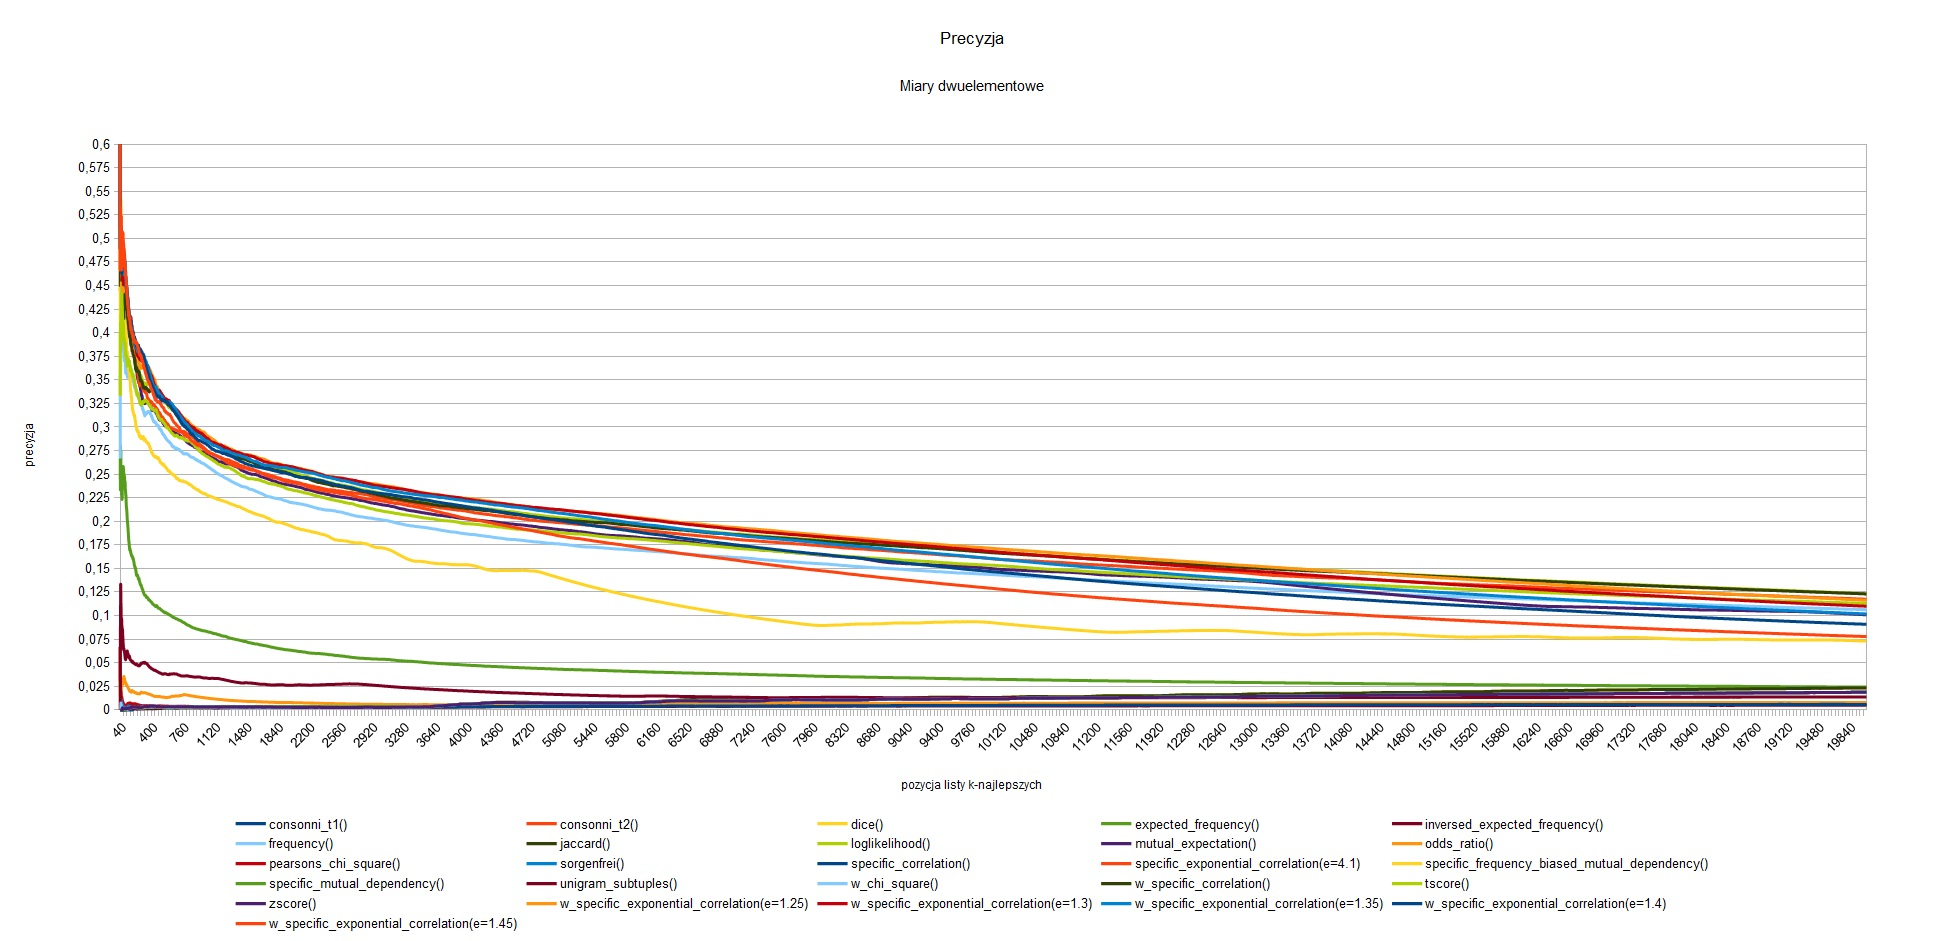
\includegraphics[width=\textwidth]{charts/wyniki_2.jpg}
\caption [Wyniki miar dwuelementowych]{Wykres prezentuje wyniki osiągnięte przez dwuelementowe miary asocjacyjne}
\label{w1}
\end{figure}

Wykres \ref{w1} prezentuje wyniki osiągnięte przez dwuelementowe miary asocjacyjne.

Najlepsze wyniki zostały osiągnięte przez następujące funkcje: \emph{W Exponential Specific Correlation} z parametrem o wartości 1.25, \emph{W Specific Correlation} oraz \emph{Loglikelihood}.


\subsubsection{Miary wieloelementowe i generalizacje funkcji dwuelementowych.}

Badanie miar trójelementowych sprowadzone zostało do wykorzystania tych samych funkcji, co w przypadku ekstrakcji kolokacji dwuelementowych, ponieważ wykorzystane zostały ich generalizacje.
Dodane do puli badanych funkcji zostały miary rozkładające $N$-elementowe kolokacje na dwuelementowe i są to \emph{Minimal bi-gram}, \emph{Average bi-gram}, \emph{Smoothed bi-gram} oraz \emph{Fair Dispersion Point Normalization}.
Jako funkcję wewnętrzną dla tych czterech funkcji wybrano \emph{W Specific Exponential Correlation} z parametrem o wartości 1.3, ponieważ generowane przez nią wyniki podczas badań nad ekstrakcją kolokacji dwuelementowych były bardzo dobre w stosunku do innych miar.
Jako badaną generalizację miary \emph{PMI} wybrano \emph{Specific Correlation}.

\begin{figure}[h!]
\centering
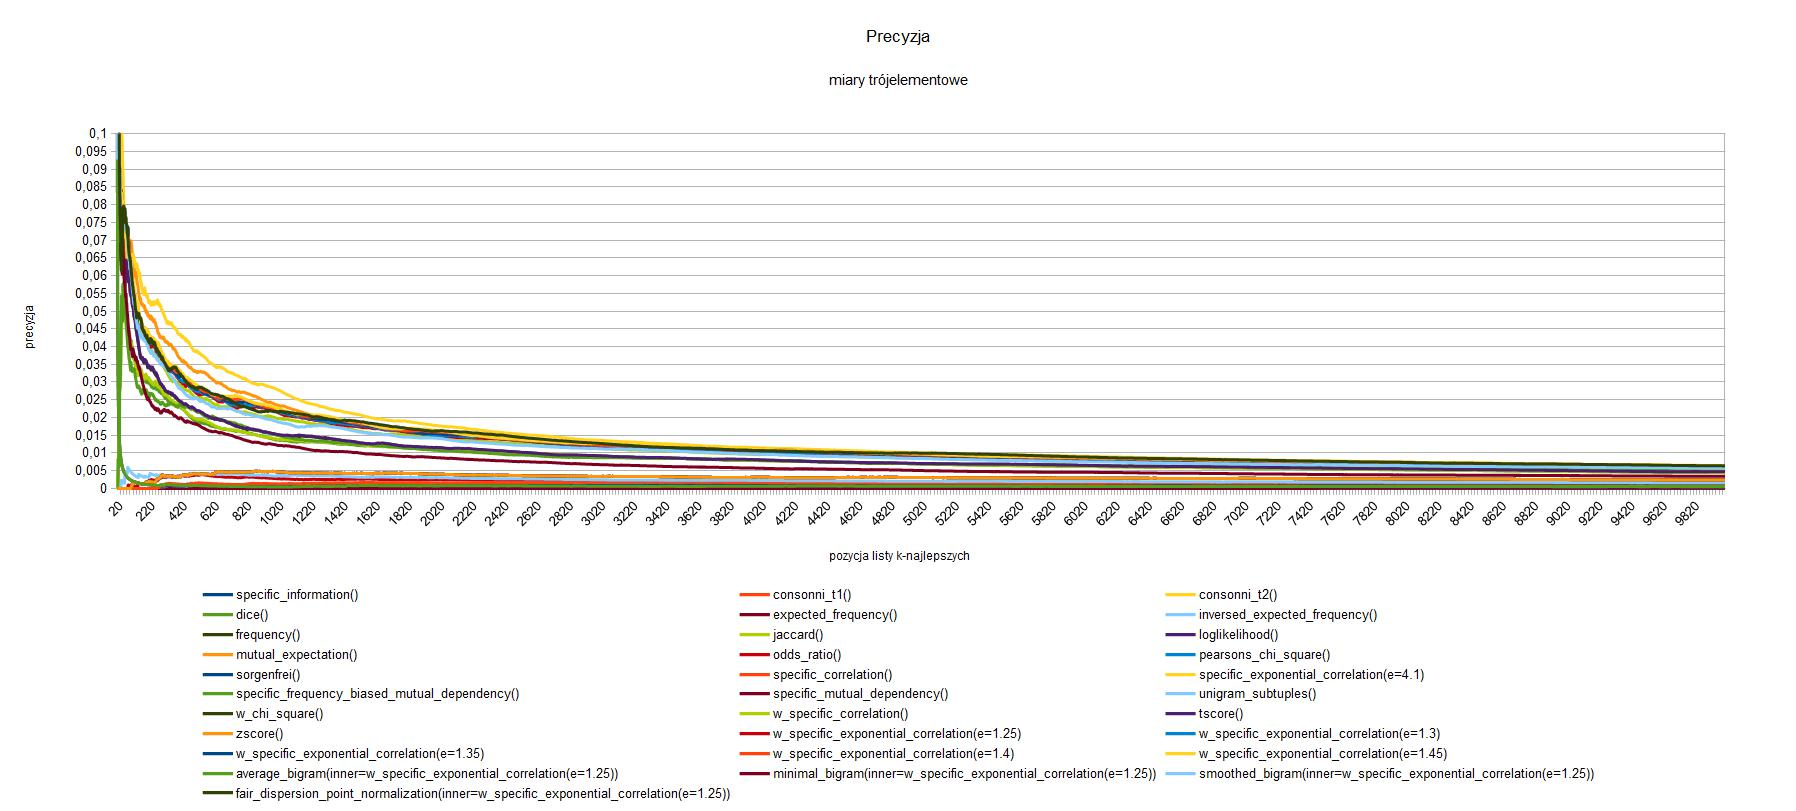
\includegraphics[width=\textwidth]{charts/wyniki_3.jpg}
\caption [Wyniki miar trójelementowych]{Wykres prezentuje wyniki osiągnięte przez trójelementowe miary asocjacyjne}
\label{w3}
\end{figure}

Wykres\ref{w3} prezentuje wyniki osiągnięte przez trójelementowe miary asocjacyjne.
Wyniki dla kolokacji trójelementowych są kilkukrotnie gorsze niż dwuelementowych, ale na uwadze trzeba mieć fakt, że zbiór wyrażeń wielowyrazowych zawiera więcej wyrażeń dwuelementowych niż trójelementowych.
Funkcje, które wygenerowały najlepsze wyniki na pozycji ok. 5000 na liście $k$-najlepszych to: \emph{Specific Exponential Correlation}, \emph{W Specific Correlation} z parametrem o wartości 1.45, \emph{Fair Dispersion Point Normalization}, a w okolicach pozycji 10000 na liście $k$-najlepszych wiele funkcji się zbiegło do podobnego wyniku.

\subsection{Podejście miar mieszanych}

Podejście miar mieszanych polegało na wykorzystaniu kombinacji liniowej rankingów wygenerowanych przez pewien zestaw poszczególnych funkcji asocjacyjnych.

\subsubsection{Optymalizacja wag dla rankingów w modelu kombinacji liniowej.}

Narzędziem wykorzystanym w optymalizacji był opisany we wcześniejszej części tej pracy algorytm ewolucyjny.
Jako zbiór uczący wybrano korpus \emph{KIPI}, a testowym był cały zbiór \emph{KGR7}.
Oba wykorzystane zbiory danych były przygotowane do tego zadania w inny sposób niż opisano w części pracy traktującej o wykorzystanych zbiorach danych.
Nie były one tagowane od nowa, a jedynie zastosowana była konwersja tagsetów z \emph{KIPI} do \emph{NKJP}.
Zauważyć jednak należy, że zarówno zbiór testowy jak i uczący były przygotowane w taki sam sposób.

Proces optymalizacji wag był wykonany dwuetapowo.
Pierwszym krokiem było dostrojenie parametrów algorytmu genetycznego, a drugim optymalizacja wag dla rankingów.
Parametry, które były optymalizowane to: szansa krzyżowania, rozmiar turnieju -- dotyczy operatora selekcji oraz szansa na mutację genotypu osobnika.
Zbadany zostały wartości parametrów przedstawione w tabeli \ref{optimizer_parameters_optimization}.
\begin{table}[h!]
\centering
\begin{tabular}{ l | c }
	\toprule
	parametr & wartości \\
	\midrule
	rozmiar turnieju & [2:5], skok co 1\\
	szansa krzyżowania & [0.4:0.8], skok co 0.05\\
	szansa mutacji & [0.03:0.11], skok co 0.01\\ 
	\bottomrule
\end{tabular}
\caption[Sprawdzone wartości parametrów algorytmu genetycznego]{Sprawdzone wartości parametrów algorytmu genetycznego}
\label{optimizer_parameters_optimization}
\end{table}

Optymalizacja parametrów algorytmu została wykonana na korpusie uczącym przy progu odcięcia na poziomie 10000 pozycji rankingu.
Każda wartość parametru była dostrajana przez 50 iteracji dla rozmiaru populacji równego 25.
Konkretny parametr był dostrajany przy utrzymaniu stałych wartości innych parametrów przez cały proces jego optymalizacji.
Ręczna ocena wyników polegała na sprawdzeniu, dla których parametrów wzrost jakości rozwiązani jest najszybszy, ale przy jednoczesnym stosunkowo powolnym zbieganiu się najlepszego, średniego i najgorszego z rozwiązań.
Ostatecznie wybrany został zestaw parametrów zaprezentowany poniżej:

\begin{table}[h!]
\centering
\begin{tabular}{ c | c | c }
	\toprule
	rozmiar turnieju & szansa krzyżowania & szansa mutacji \\
	\midrule
	5 & 0.75 & 0.05\\ 
	\bottomrule
\end{tabular}
\end{table}




Po ustaleniu parametrów dla algorytmu ewolucyjnego wykonany został drugi krok -- optymalizacja wag dla rankingów.
Optymalizacja wag rankingów polegała na wybraniu zestawu miar, które dawały dobre wyniki w ekstrakcji miar dwuelementowych, a następnie wykorzystaniu ich w procesie tworzenia rankingów do kombinacji liniowej.
Dobrane zostały następujące miary:
\begin{enumerate}
	\item \emph{Loglikelihood},
	\item \emph{Mutual Expectation},
	\item \emph{Specific Frequency Biased Mutual Dependency},
	\item \emph{Jaccard},
	\item \emph{W Specific Correlation},
	\item \emph{W Specific Exponential Correlation} z parameterami 1.35, 1.375 oraz 1.4 stosowanymi zamiennie.
\end{enumerate}


Algorytm genetyczny dostrajał wagi przeszukując przestrzeń rozwiązań, wybierając konkretny zestaw wag i sprawdzając rozwiązanie.
Zastosowany agregator to \emph{maksymalna suma}, a funkcje normalizujące to \emph{Borda score} oraz \emph{Zipf's Borda score}.
Użyta miara oceny to \emph{Average precision on hit} przy długości rankingu równej 10000.


Podjętych zostało wiele prób optymalizacji wag dla dwóch zakresów możliwych wag dla każdego z rankingu -- od 0 do 1 oraz od -1 do 1, dwóch różnych sposobów punktowania rankingów oraz dla zmiennej wartości parametru funkcji \emph{W Specific Exponential Correlation}.


\subsubsection{Wyniki i obserwacje po zastosowaniu optymalizacji. }

Badania wykazały bardzo słaby wynik dla zbioru testowego, w uczącym wynik był poprawiony o około 8\%, ale w przypadku testowego uplasował się na pozycji około 20-25\% gorszym niż najlepsze funkcje.



\section{Podsumowanie} \label{s5}

W raporcie przedstawiono koncepcję systemu do konstruowania dynamicznego słownika wielowyrazowych jednostek leksykalnych na podstawie korpusu tekstów. Opracowana metoda wydobywania jednostek wielowyrazowych składa się z 6 kroków:
\begin{enumerate}
	\item wydobycie krotek z korpusu tekstu;
	\item obliczenie dyspersji częstości dla wydobytych krotek;
	\item ekstrakcja kolokacji na podstawie wyuczonych klasyfikatorów;
	\item badania jakościowe wydobytych kolokacji;
	\item generowanie cech z wykorzystaniem miar asocjacyjnych do opisu jednostek;
	\item ekstrakcja nowych jednostek wielowyrazowych na podstawie cech uzyskanych w punkcie 5.
\end{enumerate}

Opracowane metody zostały zaimplementowane w środowisku eksperymentalnym, w którym przeprowadzono badania w zakresie zarówno strojenia licznych parametrów poszczególnych algorytmów, jak również weryfikacji jakości opracowanych metod. Pierwsze wyniki pokazały, że uzyskiwana precyzja jest bardzo wrażliwa na parametry algorytmów, dlatego niezbędne są dalsze badania.

\begin{thebibliography}{4}

\bibitem{baldwin} Baldwin, T. i Su Nam K. (2009): Multiword Expressions. In Nitin Indurkhya i Fred J. Damerau (red.) Handbook of Natural Language Processing. Second Edition, CRC Press, Boca Raton, USA.

%\bibitem{ccr}
	%Berry M. W. (2003): Survey of Text Mining - Clustering, Classification, and Retrieval.

\bibitem{broda} Broda, B., Derwojedowa, M. i Piasecki, M. (2008): Recognition of Structured Collocations in An Inflective Language. Systems Science 34, s. 27--36.

\bibitem{buczynski}	
	Buczyński A. (2004): Pozyskiwanie z Internetu tekstów do badań lingwistycznych. Praca magisterska.
	Wydział Matematyki, Informatyki i Mechaniki, 	Uniwersytet Warszawski.

\bibitem{mmi_w11}		
	Cruys T. V.: Two Multivariate Generalizations of Pointwise Mutual Information. W: Proceedings of the Workshop on Distributional Semantics and Compositionality, s. 16--20.

\bibitem{mutual_expectation}
Dias G., Lopes J. G., Guillore S. (1999): Mutual Expectation: A Measure for Multiword Lexial Unit Extraction. W: Proceedings of VEXTAL, s. 133--138.
	
%\bibitem{aggregation}		
	%Dinu A., Dinu P. L., Sorodoc I. T. (2014): Aggregation methods for efficient collocation detection.
	%University of Bucharest.

%\bibitem{evert}
	%Evert S. (2004): The Statistics of Word Cooccurrences Word Pairs and Collocations.
	%Uniwersytet Struttgart

%\bibitem{firth}
	%Firth J. R. (1957): A synopsis of linguistic theory 1930–55. In Studies in linguistic analysis.	The Philological Society, Oxford.

\bibitem{klyk}	
	Kłyk Ł. (2013): Metody sztucznej inteligencji w zwiększaniu skuteczności klasyfikatora. Praca magisterska.
	Politechnika Wrocławska, 	Wrocław.

\bibitem{hypermat}
	Lim L. H. (2013): Tensors and hypermatrices. W: Handbook of Linear Algebra pod redakcją L. Hogben (Ed.), 
	wydanie drugie, 
	CRC Press, Boca Raton.
		
\bibitem{mit} Manning Ch. D., Schütze H. (1999): Foundations of Statistical Natural Language Processing.
	Massachusetts Institute of Technology, 
	wydanie drugie.

	\bibitem{paradowski_beta}	
	Paradowski M. (2014): Opracowanie formalnej analizy zależności pomiędzy współczynnikami służącymi do wykrywania wyrażeń wielowyrazowych oraz na tej podstawie opracowanie współczynnika uogólniającego. Politechnika Wrocławska.

\bibitem{coling}
  	Pecina P., Schlesinger P. (2006): Combining Association Measures for Collocation Extraction. W: Proceedings of the COLING/ACL on Main conference poster sessions, s. 651--658.
  
\bibitem{pecina_measures}
Pecina P. (2010): Lexical association measures and collocation extraction. Language Resources and Evaluation, Volume 44, Issue 1-2, s 137--158.

%\bibitem{pecina_resource}
	%Pecina P.: Reference Data for Czech Collocation Extraction.
	%W: Proceedings of LREC workshop towards a shared task for multiword expressions, s. 11--14.

\bibitem{generalization_patterns}
	Petrovic S., Snajder J., Basic B. D. (2010): Extending lexical association measures for collocation extraction. Computer Speech \& Language, Volume 24, Issue 2, s 383--394.

	
\bibitem{wcrft} Radziszewski A. (2013): A tiered CRF tagger for Polish. Studies in Computational Intelligence 467, s. 215--230.

	 
\bibitem{wccl}
	Radziszewski A., Wardyński A., Śniatowski T. (2011): WCCL: A Morpho-syntactic Feature Toolkit. Lecture Notes in Computer Science Volume 6836, s. 434--441.
	
	\bibitem{fdpn}
	Silva J. F., Lopes G. P. (1999): A Local Maxima method and a Fair Dispersion Normalization for extracting multi-word units from corpora.
	Sixth Meeting on Mathematics of Language.

%\bibitem{smadja_xtract}
	%Smadja F. (1993): Retrieving Collocations from Text: Xtract. Journal of Computational Linguistics - Special issue on using large corpora: I archive. 
%Volume 19 Issue 1, s. 143--177. 
%MIT Press Cambridge, MA, USA.
		
\bibitem{fbmd}		
	Thanopoulos A., Fakotakis N., Kokkinakis G. (2002): Comparative Evaluation of Collocation Extraction Metrics.
	W: Proceedings of The 3rd Language Resources Evaluation Conference, s. 620--625.
	

\bibitem{kipi} http://korpus.pl/

\bibitem{slowosiec}		
	http://plwordnet.pwr.wroc.pl/wordnet/
	
\bibitem{dispersions}
	Stefan Th. Fries: Dispersions and adjusted frequencies in corpora.
	University of California, Santa Barbara.


\end{thebibliography}
\end{document}
